\input{setup.tex}

% Режим шаблона (должен быть включен один из трех)
\ВКРtrue
%\Практикаtrue
%\Курсоваяtrue

\newcommand{\Дисциплина}{<<Проектирование и архитектура программных систем>>} % для курсовой
\newcommand{\КодСпециальности}{09.03.04} % Курсовая
\newcommand{\Специальность}{Программная инженерия} % Курсовая
\newcommand{\Тема}{Программно-информационная система управления книжным магазином} % ВКР Курсовая
\newcommand{\ТемаВтораяСтрока}{}
\newcommand{\ГдеПроводитсяПрактика}{ООО <<Предприятие ВТИ-Сервис>>} % для практики
\newcommand{\РуководительПрактПредпр}{Федосов Д. В.} % для практики
\newcommand{\ДолжнРуководительПрактПредпр}{директор} % для практики
\newcommand{\РуководительПрактУнивер}{Чаплыгин А. А.} % для практики
\newcommand{\ДолжнРуководительПрактУнивер}{к.т.н. доцент} % для практики
\newcommand{\Автор}{Д. Н. Рязанцев}
\newcommand{\АвторРод}{Рязанцева Д. Н.}
\newcommand{\АвторПолностьюРод}{Рязанцева Даниила Николаевича} % для практики
\newcommand{\Шифр}{21-06-0011}
\newcommand{\Курс}{4 } % для практики
\newcommand{\Группа}{ПО-11б}
\newcommand{\Руководитель}{Е. П. Кочура} % для ВКР и курсовой
\newcommand{\Нормоконтроль}{А. А. Чаплыгин} % для ВКР
\newcommand{\ЗавКаф}{А. В. Малышев} % для ВКР
\newcommand{\ДатаПриказа}{«04» апреля 2025~г.} % для ВКР
\newcommand{\НомерПриказа}{1696-с} % для ВКР
\newcommand{\СрокПредоставления}{«9» июня 2025~г.} % для ВКР, курсового

\begin{document}
	\maketitle
	\ifПрактика{}\else{
		\input{ЛистЗадания}
		\abstract{РЕФЕРАТ}

Объем работы равен \formbytotal{lastpage}{страниц}{е}{ам}{ам}. Работа содержит \formbytotal{figurecnt}{иллюстраци}{ю}{и}{й}, \formbytotal{tablecnt}{таблиц}{у}{ы}{}, \arabic{bibcount} библиографических источников и \formbytotal{числоПлакатов}{лист}{}{а}{ов} графического материала. Количество приложений – 2. Графический материал представлен в приложении А. Фрагменты исходного кода представлены в приложении Б.

Перечень ключевых слов: интернет-магазин, веб-приложение, база данных, Flask, JavaScript, HTML, CSS, PostgreSQL, аутентификация, авторизация, каталог книг, заказы, пользователи, REST API.

Объектом разработки является программно-информационная система управления книжным магазином, реализованная в виде веб-приложения с клиент-серверной архитектурой.

Целью выпускной квалификационной работы является разработка веб-приложения для автоматизации процессов управления книжным магазином, включая просмотр каталога, оформление заказов и администрирование данных.

В процессе разработки были определены основные сущности системы (книги, авторы, жанры, пользователи, заказы), спроектирована реляционная база данных PostgreSQL, реализованы серверная часть на Python с использованием Flask и клиентская часть с применением HTML, CSS и JavaScript. Система поддерживает функционал для трех ролей пользователей: покупатель, сотрудник, администратор. Разработан адаптивный пользовательский интерфейс, обеспечивающий удобство работы на различных устройствах. Проведено тестирование системы для подтверждения ее работоспособности.

\selectlanguage{english}
\abstract{ABSTRACT}
  
The volume of work is \formbytotal{lastpage}{page}{}{s}{s}. The work contains \formbytotal{figurecnt}{illustration}{}{s}{s}, \formbytotal{tablecnt}{table}{}{s}{s}, \arabic{bibcount} bibliographic sources and \formbytotal{числоПлакатов}{sheet}{}{s}{s} of graphic material. The number of applications is 2. The graphic material is presented in annex A. The layout of the site, including the connection of components, is presented in annex B.

List of keywords: online store, web application, database, Flask, JavaScript, HTML, CSS, PostgreSQL, authentication, authorization, book catalog, orders, users, REST API.

Object of development: a software-information system for managing a bookstore, implemented as a web application with a client-server architecture.

Purpose of the final qualifying work: to develop a web application for automating bookstore management processes, including browsing the catalog, placing orders, and administering data.

Development process: the main system entities (books, authors, genres, users, orders) were defined, a relational PostgreSQL database was designed, the server-side was implemented using Python with Flask, and the client-side was developed using HTML, CSS, and JavaScript. The system supports functionality for three user roles: customer, employee, and administrator. An adaptive user interface was created to ensure usability across various devices. System testing was conducted to confirm its functionality.
\selectlanguage{russian}
}\fi
	\tableofcontents
	\section*{ОБОЗНАЧЕНИЯ И СОКРАЩЕНИЯ}

БД -- база данных.

ИС -- информационная система.

ИТ -- информационные технологии. 

ПО -- программное обеспечение.

РП -- рабочий проект.

СУБД -- система управления базами данных.

ТЗ -- техническое задание.

ТП -- технический проект.

UML (Unified Modelling Language) -- язык графического описания для объектного моделирования в области разработки программного обеспечения.

REST (Representational State Transfer) -- архитектурный стиль для веб-сервисов.

UI (User Interface) -- пользовательский интерфейс.
	\ifПрактика{}\else{\section*{ВВЕДЕНИЕ}
\addcontentsline{toc}{section}{ВВЕДЕНИЕ}

Современные информационные технологии играют ключевую роль в развитии бизнеса, особенно в сфере розничной торговли. Интернет-магазины стали важным инструментом для взаимодействия с клиентами, предоставляя удобный доступ к товарам и услугам в любое время и из любой точки мира. В книжной индустрии онлайн-торговля позволяет не только расширить ассортимент, но и автоматизировать процессы управления, упрощая работу как для покупателей, так и для сотрудников магазина. Разработка веб-приложений для таких задач требует применения современных технологий, обеспечивающих надежность, масштабируемость и удобство использования.

Создание программно-информационной системы для управления книжным магазином позволяет оптимизировать процессы обработки заказов, ведения каталога книг и взаимодействия с клиентами. Такая система предоставляет покупателям возможность просматривать книги, оформлять заказы и отслеживать их статус, а сотрудникам и администраторам — эффективно управлять ассортиментом и данными пользователей.

\emph{Цель настоящей работы} – разработка веб-приложения для автоматизации управления книжным магазином, обеспечивающего удобный интерфейс для клиентов и функционал для администрирования. Для достижения цели необходимо решить \emph{следующие задачи:}
\begin{itemize}
\item провести анализ предметной области интернет-торговли книгами;
\item разработать концептуальную модель системы управления книжным магазином;
\item спроектировать программную систему;
\item реализовать и протестировать веб-приложение с использованием веб-технологий.
\end{itemize}

\emph{Структура и объем работы.} Отчет состоит из введения, 4 разделов основной части, заключения, списка использованных источников, 2 приложений. Текст выпускной квалификационной работы равен \formbytotal{lastpage}{страниц}{е}{ам}{ам}.

\emph{Во введении} сформулирована цель работы, поставлены задачи разработки, описана структура работы, приведено краткое содержание каждого из разделов.

\emph{В первом разделе} на стадии описания технической характеристики предметной области приводится анализ предметной области, включая особенности интернет-торговли книгами и требования к системе.

\emph{Во втором разделе} на стадии технического задания приводятся требования к разрабатываемой системе.

\emph{В третьем разделе} на стадии технического проектирования представлен технический проект, включая выбор технологий, проектирование архитектуры и пользовательского интерфейса.

\emph{В четвертом разделе} приводится список модулей и их методов, использованных при разработке системы, производится тестирование разработанного сайта.

В заключении излагаются основные результаты работы, полученные в ходе разработки.

В приложении А представлен графический материал.
В приложении Б представлены фрагменты исходного кода. 
}\fi
	\section{Анализ предметной области}
\subsection{Понятие и ключевые аспекты интернет-торговли}

Интернет-торговля (или электронная коммерция) – это форма коммерческой деятельности, при которой сделки купли-продажи товаров, услуг или цифровых продуктов осуществляются через интернет с использованием электронных платежных систем и цифровых коммуникационных каналов \cite{1}.
Из этого термина можно выделить две основные концепции интернет-торговли:

\begin{enumerate}
	\item Широкий подход – интернет-торговля рассматривается как синоним электронной коммерции, охватывающей все аспекты бизнеса: маркетинг, логистику, платежи, CRM-системы и послепродажное обслуживание.
	\item Узкий подход – интернет-торговля трактуется как частный случай электронной коммерции, ограниченный дистанционной продажей товаров через интернет.
\end{enumerate}

В статье «Развитие электронной торговли в Российской Федерации» С.С. Корнева выделяет девять ключевых форм электронной коммерции, классифицируемых по типу взаимодействия участников сделки \cite{2}.:
\begin{itemize}
	\item B2B (Business-to-Business) – сделки между коммерческими организациями. Включает корпоративные электронные рынки и внутренние системы управления предприятием. На эту модель приходится наибольший объём электронных сделок;
	\item B2C (Business-to-Consumer) – продажи товаров и услуг от бизнеса конечным потребителям. К такой форме относятся интернет-магазины (Ozon, Citilink) и разного рода онлайн-услуги (образование, страхование, банкинг);
	\item B2G (Business-to-Government) – государство предоставляет бизнесу услуги (налоги, лицензирование, закупки) в электронном формате;
	\item C2C (Consumer-to-Consumer) – торговля между частными лицами через онлайн-платформы. Яркими представителями такой интернет-торговли являются доски объявлений (Avito);
	\item C2B (Consumer-to-Business) – частные лица предлагают товары/услуги компаниям. К таким, например, относятся краудсорсинговые платформы (Planeta, Kickstarter);
	\item C2G (Consumer-to-Government) – частные лица участвуют в сделке с правительственной структуре, производят выплаты по счетам;
	\item G2C (Government-to-Consumer) – взаимодействие государства с гражданами через цифровые сервисы, например, выплаты пособий (Госуслуги);
	\item G2B (Government-to-Business) – государство предоставляет бизнесу услуги (налоги, лицензирование) в электронном формате;
	\item G2G (Government-to-Government) – электронный документооборот между госучреждениями; 
 \end{itemize}
 
На данный момент доминирующими формами являются B2B и B2G \cite{2}.
Интернет-торговля обладает рядом значительных преимуществ по сравнению с традиционной розничной торговлей. Эти преимущества касаются как бизнеса, так и потребителей, а также способствуют развитию экономики в целом.

Для бизнеса можно выделить следующие основные выгоды:
 \begin{itemize}
 	\item глобальный охват рынка. Интернет-магазин доступен круглосуточно из любой точки мира, что позволяет привлекать клиентов за пределами локального рынка;
 	\item снижение операционных затрат. Отсутствие расходов на аренду торговых площадей, коммунальные услуги и большое количество персонала. Автоматизация процессов (учёт товаров, обработка заказов, CRM-системы) сокращает издержки;
 	\item упрощение логистики и автоматизация. Интеграция с курьерскими службами и маркетплейсами ускоряет доставку.
 \end{itemize}
 
 Для потребителей:
 \begin{itemize}
 	\item удобство и экономия времени. Покупки в любое время суток без необходимости посещения магазинов, доступ к широкому ассортименту товаров и сравнение цен в несколько кликов;
 	\item возможность возврата и гарантийного обслуживания. Законодательство о дистанционной торговле защищает права покупателей (например, право на возврат в течение 7 дней) \cite{3}, упрощённые процедуры обмена и возврата через онлайн-поддержку;
 	\item доступ к скидкам и акциям. Купоны, кэшбэк, программы лояльности и подписки (например, Wildberries Premium), алгоритмы персонализированных предложений на основе истории покупок.
 \end{itemize}
 
 Для экономики и общества:
 \begin{itemize}
 	\item стимулирование цифровизации. Развитие ИТ-инфраструктуры, платежных систем и логистических сервисов, создание новых рабочих мест (разработчики, маркетологи, курьерские службы);
 	\item поддержка малого бизнеса. Низкий порог входа для стартапов (можно начать с маркетплейсов или соцсетей), Доступ к инструментам продвижения (таргетированная реклама, SEO).
 \end{itemize}
 
 Интернет-торговля предлагает выгоды для всех участников рынка. Её развитие продолжает трансформировать розничную торговлю, делая её более эффективной и клиентоориентированной.
 
\subsubsection{Интернет-магазины как ключевая форма интернет-торговли}

Интернет-магазин — это виртуальная торговая площадка, функционирующая на базе интернет-технологий, где покупатели могут выбирать, заказывать и оплачивать товары или услуги онлайн. В отличие от традиционной розничной торговли, интернет-магазин не требует физического присутствия покупателя и продавца в одном месте, что значительно расширяет географию продаж и снижает издержки.

Ключевые особенности интернет-магазинов:
 \begin{itemize}
 	\item электронная витрина — веб-сайт с каталогом товаров, подробными описаниями, изображениями и ценами;
 	\item торговая система — автоматизированные процессы оформления заказа, оплаты и доставки;
 	\item корзина покупок — функционал, позволяющий пользователю собирать выбранные товары и редактировать заказ перед оплатой.
 \end{itemize}
 
 Интернет-магазины представляют собой динамично развивающийся сегмент электронной коммерции, сочетающий технологические инновации с удобством для потребителей. Их дальнейший рост будет зависеть от адаптации к изменяющимся рыночным условиям и внедрения новых цифровых решений \cite{4}.
 
\subsubsection{Интернет-торговля в современном бизнесе}

Интернет-торговля кардинально изменила подходы к ведению бизнеса, создав новые возможности для компаний различных масштабов. Её роль в современной экономике невозможно переоценить, так как она позволяет выходить на глобальные рынки, оптимизировать издержки и выстраивать эффективные коммуникации с потребителями \cite{5}.

Одним из ключевых преимуществ интернет-торговли для бизнеса является доступ к международным рынкам без необходимости открытия физических представительств. Российские компании, такие как Wildberries и Ozon, успешно используют этот потенциал, расширяя своё присутствие за рубежом. Кроме того, онлайн-формат торговли значительно снижает операционные затраты за счёт экономии на аренде помещений, содержании персонала и других традиционных статьях расходов. Автоматизация бизнес-процессов с помощью CRM и ERP-систем дополнительно повышает эффективность управления.

Гибкость интернет-торговли позволяет компаниям быстро адаптироваться к изменениям спроса, тестировать новые продукты и масштабировать бизнес с минимальными рисками. Персонализация взаимодействия с клиентами, основанная на анализе данных, даёт возможность предлагать индивидуальные решения и повышать лояльность аудитории. Круглосуточная доступность онлайн-магазинов обеспечивает стабильный поток продаж без временных ограничений.

Влияние интернет-торговли на экономику проявляется в её растущем вкладе в ВВП. Согласно исследованиям, объём рынка электронной коммерции в России увеличился с 1,7 трлн рублей в 2017 году до 8 трлн рублей в 2020 году \cite{6}. Этот рост сопровождается созданием новых рабочих мест в сферах логистики, ИТ и цифрового маркетинга, а также стимулированием малого бизнеса, для которого онлайн-платформы стали доступным инструментом выхода на рынок.

Однако развитие интернет-торговли сопряжено с рядом вызовов. Высокая конкуренция, особенно со стороны международных гигантов, таких как Amazon и Aliexpress, требует от компаний инновационных решений. Логистические сложности, особенно в удалённых регионах, и недостаточная развитость инфраструктуры также остаются серьёзными барьерами. Правовые риски, связанные с отсутствием единого регулирования, и угрозы кибербезопасности добавляют неопределённости в работу онлайн-бизнеса.

Перспективы развития интернет-торговли связаны с внедрением передовых технологий, таких как дополненная и виртуальная реальность для виртуальных примерок, а также голосовая коммерция. Важную роль играет государственная поддержка, включая меры по легализации отрасли, развитию цифровой инфраструктуры и созданию благоприятных налоговых условий.
Таким образом, интернет-торговля продолжает трансформировать бизнес-среду, предлагая компаниям инструменты для роста и повышения конкурентоспособности. Для устойчивого развития отрасли необходимо решать существующие задачи, включая вопросы регулирования, логистики и технологий, чтобы максимально реализовать её потенциал в экономике будущего \cite{5}.



\subsubsection{Интернет-торговля для потребителя}

Интернет-торговля кардинально изменила потребительское поведение, предоставив покупателям новые возможности и изменив их подход к совершению покупок. Как отмечает Воскресенская О.В., онлайн-магазины стали не просто альтернативой традиционной розничной торговле, а основным каналом удовлетворения потребностей современного потребителя \cite{7}.

Онлайн-площадки обеспечивают потребителям круглосуточный доступ к товарам и услугам, позволяя совершать покупки в любое время и из любой точки мира. Это особенно важно в условиях глобализации, когда покупатели могут выбирать товары не только у локальных продавцов, но и у международных поставщиков \cite{8}.

Интернет-магазины предлагают значительно более широкий ассортимент по сравнению с физическими магазинами. Потребители могут легко сравнивать цены, читать отзывы и изучать характеристики товаров перед покупкой.

Просмотр товаров онлайн стал формой развлечения, что увеличивает частоту покупок, а изобилие аналогов учит потребителей более внимательно оценивать качество и стоимость товаров.

Интернет-торговля трансформировала потребительское поведение, сделав покупки более удобными, но и более сложными с точки зрения контроля расходов. Её дальнейшее развитие потребует баланса между удобством, прозрачностью и защитой прав покупателей.

\subsection {История интернет-торговли}
Интернет-торговля зародилась задолго до появления современных онлайн-магазинов. Первые шаги были связаны с электронным обменом данными между компаниями, но настоящий прорыв произошел с распространением интернета.

Сначала онлайн-продажи ограничивались простыми товарами, такими как книги и техника. Постепенно компании начали разрабатывать удобные платформы, системы оплаты и доставки, что сделало интернет-торговлю доступной для массового потребителя.

Со временем ассортимент расширился до практически любых товаров и услуг, а технологии персонализации и маркетинга позволили делать покупки в интернете еще удобнее. Сегодня интернет-торговля — это глобальная индустрия, которая продолжает развиваться, внедряя новые технологии, такие как мобильные платежи, искусственный интеллект и быструю доставку.

\subsubsection{Мировая история развития интернет-торговли}

Развитие интернет-торговли представляет собой многогранную историю технологического прогресса, которая коренным образом изменила мировую экономику и потребительские привычки. Ее становление можно проследить через несколько ключевых этапов.

Первые шаги электронной коммерции были сделаны еще в 1960 году, когда компании IBM и American Airlines разработали инновационную систему для бронирования авиабилетов. Этот проект стал прообразом современных онлайн-транзакций. В 1970-1980-х годах началось активное внедрение систем электронного обмена данными (EDI), что позволило автоматизировать бизнес-процессы в логистике и оптовой торговле. Важным рубежом стал 1989 год, когда интернет приобрел современные черты с появлением стандартов HTTP, что открыло новые возможности для онлайн-коммерции  \cite{9}.

Настоящий прорыв произошел в 1990-х годах, когда в США были сняты ограничения на коммерческое использование интернета. Это десятилетие ознаменовалось появлением пионеров электронной коммерции: в 1994 году была создана первая платежная система CyberCash, в 1995 году Джефф Безос основал Amazon, начавший с продажи книг и превратившийся в крупнейший мировой маркетплейс. Тогда же появился eBay, революционизировавший торговлю через онлайн-аукционы. Эти платформы заложили основы современных моделей B2C и C2C \cite{9}.

\subsubsection{Развитие интернет-торговли в России}

В России интернет-торговля начала развиваться после распада СССР. Первые сделки в 1990-х осуществлялись по системе MOTO (заказ по телефону с последующей почтовой доставкой). На рубеже веков появились первые российские интернет-магазины, к 2020 году весомый процент продаж приходился на маркетплейсы Ozon и Wildberries.

Современный этап характеризуется доминированием маркетплейсов, объединяющих миллионы продавцов и покупателей. Особое значение приобрела мобильная коммерция - по данным исследований, более 60\% покупок сейчас совершается через смартфоны. Российские площадки, успешно выходят на международные рынки, демонстрируя глобализацию электронной торговли \cite{10}.

\subsubsection{Влияние пандемии COVID-19 на интернет-торговлю}

Пандемия COVID-19 стала мощным катализатором для ускоренного развития интернет-торговли, коренным образом изменив потребительские привычки и структуру рынка. По данным исследования, в 2020 году российский рынок онлайн-торговли вырос на 57\%, достигнув объема 2,7 трлн рублей, при этом наиболее значительный рост (на 172\%) наблюдался в сегменте пищевых продуктов. Это было обусловлено вынужденным переходом потребителей на онлайн-шопинг из-за карантинных ограничений \cite{11}.

Ключевые изменения, вызванные пандемией:
\begin{enumerate}
	\item Расширение аудитории:
	\begin{itemize}
		\item прирост пользователей онлайн-торговли составил 10 млн человек, включая ранее неактивную возрастную группу 55+;
		\item увеличилась частота покупок: 45\% респондентов отметили рост повторных заказов.
	\end{itemize}
	
	\item Трансформация логистики:
	\begin{itemize}
		\item бесконтактная доставка (94\% спроса);
		\item самовывоз из магазинов (65\%);
		\item партнерства с курьерскими сервисами и такси для снижения нагрузки на склады.
	\end{itemize}
	
	\item Технологический прорыв:
	\begin{itemize}
		\item 65\% компаний столкнулись с перебоями в ИТ-системах, что стимулировало внедрение решений для масштабирования;
		\item реклама в соцсетях: 20\% бизнесов начали использовать ее впервые.
	\end{itemize}
	
	\item Сдвиг в товарных категориях:
	\begin{itemize}
		\item рост спроса на продукты питания и товары первой необходимости;
		\item снижение продаж одежды и дорогой техники из-за экономической нестабильности.
	\end{itemize}
	
	\item Долгосрочные последствия:
	\begin{itemize}
		\item онлайн-торговля стала дополнять офлайн, а не заменять его: 45\% респондентов считают, что физические магазины сохранят актуальность.
		\item развитие маркетплейсов как ключевого канала сбыта для производителей.
	\end{itemize}
	
\end{enumerate}

COVID-19 не только ускорил цифровизацию торговли, но и выявил ее уязвимости, заставив бизнес адаптироваться.


\subsection{Интернет-торговля книгами}

Интернет-торговля книгами является одним из ключевых направлений развития электронной коммерции. Зарубежный опыт, в частности успех компании Amazon.com, демонстрирует эффективность сочетания инновационных технологий, клиентоориентированного подхода и широкого ассортимента. Amazon.com достигла высоких показателей за счет персонализации сервиса, удобной навигации, системы рекомендаций и быстрой доставки, что позволило ей завоевать доверие миллионов покупателей.

В России данный сегмент также развивается, однако существуют значительные отличия от зарубежных стандартов. Крупнейшие российские книжные интернет-магазины, такие как Ozon, Labirint, Bolero и Книга.ру, пока не могут конкурировать с Amazon.com по уровню сервиса, логистики и масштабам деятельности \cite{12}. Среди основных проблем российского рынка можно выделить:
\begin{itemize}
	\item ограниченный ассортимент электронных книг;
	\item высокие тарифы на доставку, особенно в регионы;
	\item низкую скорость выполнения заказов;
	\item недоверие покупателей к онлайн-продавцам из-за некорректного указания цен и отсутствия товаров в наличии.
\end{itemize}

Для дальнейшего развития интернет-торговли книгами в России необходимо внедрение современных логистических решений, улучшение качества обслуживания клиентов и расширение ассортимента, включая цифровые форматы. Опыт Amazon.com может служить ориентиром для российских компаний, стремящихся повысить конкурентоспособность на международном рынке.
	\section{Техническое задание}
\subsection{Основание для разработки}

Основанием для разработки является задание на выпускную квалификационную работу бакалавра.

 Полное наименование системы: «Программно-информационная система управления книжным магазином».

\subsection{Цель и назначение разработки}

Разрабатываемая программно-информационная система предназначена для управления ассортиментом книг, обработки заказов, предоставления удобного интерфейса покупателям и сотрудникам.

Программа ориентирована на предпринимателей, планирующих в будущем выходить на всероссийский рынок.

Задачами данной разработки являются:
\begin{enumerate}
\item Создание серверной части на Flask для обработки запросов и взаимодействия с базой данных PostgreSQL.
\item Разработка клиентской части на HTML, CSS и JavaScript для отображения книг, корзины и управления заказами.
\item Реализация системы аутентификации и авторизации пользователей с разными ролями (клиент, сотрудник, администратор).
\item Интеграция механизмов поиска и пагинации для удобного просмотра каталога книг.
\end{enumerate}


\subsection{Требования к программной системе}


\subsubsection{Требования к данным программной системы}


На рисунке 2.1 представлена модель данных программной системы в виде UML-диаграммы сущность-связь.


\begin{figure}[H]
	\centering
	\includegraphics[width=0.7\linewidth]{"images/Модель_данных"}
	\caption{Модель данных}
	\label{fig:--}
\end{figure}

Входными данными системы являются:
\begin{itemize}
	\item сведения о книгах;
	\item параметры корзины
	\item учётные данные пользователя
\end{itemize}

Выходными данными являются:
\begin{itemize}
	\item идентификаторы оформленных заказов
	\item уведомления о статусе заказов
\end{itemize}



Программно-информационная система должна обеспечивать хранение и обновление данных о книгах, пользователях и заказах.

\subsubsection{Функциональные требования к программной системе}

Разрабатываемая программно-информационная система книжного магазина предусматривает три роли пользователей: покупатели, сотрудники и администраторы. Каждой роли доступны определенные функции.

Для всех пользователей:

\begin{enumerate}
	\item Просмотр каталога книг:
	\begin{itemize}
		\item отображение списка книг с возможностью сортировки и фильтрации;
		\item поиск книг по названию, автору или жанру.
	\end{itemize}
	\item Просмотр деталей книги:
	\begin{itemize}
		\item информация о названии, авторе, цене, наличии на складе и описании.
	\end{itemize}
	\item Авторизация и регистрация:
	\begin{itemize}
		\item вход в систему под своей учетной записью;
		\item создание нового аккаунта.
	\end{itemize}
\end{enumerate}

Для зарегистрированных покупателей:
\begin{enumerate}
	\item Оформление заказов:
	\begin{itemize}
		\item подтверждение заказа с указанием итоговой суммы;
	\end{itemize}
	\item Просмотр истории заказов:
	\begin{itemize}
		\item отслеживание своих заказов;
		\item отслеживание текущего статуса заказов.
	\end{itemize}
\end{enumerate}

Для сотрудников:
\begin{enumerate}
	\item Управление книгами:
	\begin{itemize}
		\item добавление новых книг в каталог;
		\item редактирование информации о существующих книгах;
		\item удаление книг из каталога.
	\end{itemize}
	\item Управление заказами:
	\begin{itemize}
		\item просмотр всех заказов;
		\item изменение статуса заказов.
	\end{itemize}
\end{enumerate}

Для администраторов:
\begin{enumerate}
	\item Управление пользователями:
	\begin{itemize}
		\item назначение ролей;
		\item просмотр списка всех пользователей.
	\end{itemize}
	\item Полный доступ к функциям сотрудников:
	\begin{itemize}
		\item просмотр всех заказов;
		\item все возможности сотрудников, включая управление книгами и заказами.
	\end{itemize}
\end{enumerate}

На рисунке 2.2 в виде диаграммы прецедентов представлены функциональные требования к системе, доступные для всех категорий пользователей.

На рисунке 2.3 представлены дополнительные функциональные требования к системе для авторизованных.

На рисунке 2.4 представлены дополнительные функциональные требования к системе для пользователей с ролью сотрудника.

На рисунке 2.5 представлены дополнительные функциональные требования к системе для пользователей с ролью администратора.

\begin{figure}[H]
	\centering
	\includegraphics[width=0.7\linewidth]{"images/Все_пользователи"}
	\caption{Диаграмма прецедентов для неавторизованных пользователей}
	\label{fig:--}
\end{figure}

\begin{figure}[H]
	\centering
	\includegraphics[width=0.7\linewidth]{"images/Авторизованные"}
	\caption{Диаграмма прецедентов для авторизованных пользователей}
	\label{fig:--}
\end{figure}

\begin{figure}[H]
	\centering
	\includegraphics[width=0.7\linewidth]{"images/Сотрудники"}
	\caption{Диаграмма прецедентов для пользователей с ролью сотрудника}
	\label{fig:--}
\end{figure}

\begin{figure}[H]
	\centering
	\includegraphics[width=0.7\linewidth]{"images/Администраторы"}
	\caption{Диаграмма прецедентов для пользователей с ролью администратора}
	\label{fig:--}
\end{figure}


\paragraph{Вариант использования «Просмотр каталога книг»}

Заинтересованные лица и их требования: покупатель, гость сайта, желает ознакомиться с ассортиментом книг интернет-магазина.

Предусловие: открыта главная страница сайта.

Постусловие: пользователь видит список книг.

Основной успешный сценарий:

\begin{enumerate}
	\item Пользователь заходит на сайт
	\item Приложение загружает список книг с пагинацией (по 8 книг на страницу).
\end{enumerate}


\paragraph{Вариант использования «Поиск книг»}

Заинтересованные лица и их требования: пользователь желает найти конкретную книгу.

Предусловие: открыта главная страница сайта.

Постусловие: пользователь находит или не находит нужную ему книгу.

Основной успешный сценарий:

\begin{enumerate}
	\item Пользователь пишет полное название книги или её часть в поле поиска.
	\item Приложение отправляет запрос к API. 
	\item Сервер возвращает книги, название которых соответствуют поисковому запросу.
	\item Пользователь может переключать страницы с результатами.
\end{enumerate}


\paragraph{Вариант использования «Просмотр деталей книги» }

Заинтересованные лица и их требования: покупатель, желающий узнать подробности о книге.

Предусловие: открыта главная страница сайта.

Постусловие: пользователь видит полную информацию о книге.

Основной успешный сценарий:

\begin{enumerate}
	\item Пользователь нажимает на кнопку "Подробнее".
	\item Приложение отправляет запрос к API для получения полной информации о книге.
	\item Открывается модальное окно с деталями: автор, цена, описание, жанры и т.д.
	\item Пользователь может закрыть окно или добавить книгу в корзину.
\end{enumerate}


\paragraph{Вариант использования «Добавление книги в корзину»}

Заинтересованные лица и их требования: покупатель, который авторизован на сайте, желает добавить книгу в корзину.

Предусловие: пользователь авторизован и открыта главная страница сайта.

Постусловие: книга добавлена в корзину.

Основной успешный сценарий:

\begin{enumerate}
	\item Пользователь нажимает кнопку "В корзину" на карточке книги.
	\item Если пользователь не авторизован, появляется уведомление с предложением войти.
	\item Книга добавляется в корзину (локальное хранилище и состояние UI обновляются).
	\item Кнопка меняется на "В корзине" и становится неактивной.
	\item Появляется возможность нажать кнопку "Оформить заказ"
	и отображается стоимость корзины.
\end{enumerate}


\paragraph{Вариант использования «Управление корзиной»}

Заинтересованные лица и их требования: авторизованный покупатель желает изменить свою корзину.

Предусловие: в корзине есть хотя бы один товар и открыта главная страница сайта.

Постусловие: состояние корзины обновлено.

Основной успешный сценарий:

\begin{enumerate}
	\item Пользователь спускается в корзину.
	\item Пользователь может увеличить или уменьшить количество выбранных книг.
	\item Пользователь может выборочно удалить книги из корзины.
	\item Обновляется общая стоимость заказа.
	\item Если товара нет в достаточном количестве, отображается предупреждение.
	\item При соблюдении условий становится доступна кнопка "Оформить заказ".
\end{enumerate}


\paragraph{Вариант использования «Оформление заказа»}

Заинтересованные лица и их требования: авторизованный покупатель, который желает заказать книги из корзины.

Предусловие: открыта главная страница сайта, есть книги в корзине и выбрано имеющееся на складе их количество.

Постусловие: заказ создан, корзина очищена.

Основной успешный сценарий:

\begin{enumerate}
	\item Пользователь нажимает "Оформить заказ".
	\item Приложение отправляет на сервер данные о заказе.
	\item Сервер проверяет наличие товаров и создает заказ.
	\item Пользователь получает уведомление об успешном оформлении с номером заказа и деталями.
	\item Корзина очищается.
\end{enumerate}


\paragraph{Вариант использования «Просмотр истории заказов»}

Заинтересованные лица и их требования: авторизованный покупатель, желает посмотреть на историю заказов.

Предусловие: пользователь авторизован и открыта главная страница сайта

Постусловие: отображается список заказов.

Основной успешный сценарий:

\begin{enumerate}
	\item Пользователь нажимает "Мои заказы".
	\item Приложение загружает список заказов через API.
	\item При наличии заказов для каждого отображаются номер, дата, статус, сумма.
\end{enumerate}


\paragraph{Вариант использования «Просмотр подробностей заказа»}

Заинтересованные лица и их требования: авторизованный покупатель желает подробнее изучить свой заказ.

Предусловие: пользователь авторизован, на главной странице и имеет хотя бы один заказ.

Постусловие: пользователь узнаёт подробности своего заказа.

Основной успешный сценарий:

\begin{enumerate}
	\item Пользователь нажимает "Мои заказы".
	\item Приложение загружает список заказов через API.
	\item Пользователь нажимает на один из своих заказов.
	\item При наличии этих книг в системе пользователь увидит сколько он заказал определённых книг и их стоимость по отдельности.
\end{enumerate}


\paragraph{Вариант использования «Просмотр истории заказов сотрудником или администратором»}

Заинтересованные лица и их требования: пользователь авторизованный на аккаунте с ролью сотрудника или администратора желает посмотреть список заказов всех пользователей.

Предусловие: пользователь авторизован, его аккаунт имеет роль сотрудника или администратора и открыта главная страница сайта.

Постусловие: пользователь видит список всех заказов.

Основной успешный сценарий:

\begin{enumerate}
	\item Пользователь нажимает "Все заказы".
	\item Приложение загружает список заказов через API.
	\item При наличии заказов для каждого отображаются номер, дата, статус, сумма.
\end{enumerate}


\paragraph{Вариант использования «Просмотр подробностей заказа сотрудником или администратором»}

Заинтересованные лица и их требования: пользователь авторизованный на аккаунте с ролью сотрудника или администратора желает посмотреть подробности заказа одного из пользователей.

Предусловие: пользователь авторизован, его аккаунт имеет роль сотрудника или администратора и открыта главная страница сайта.

Постусловие: пользователь узнаёт подробности заказа одного из пользователей.

Основной успешный сценарий:

\begin{enumerate}
	\item Пользователь нажимает "Все заказы".
	\item Приложение загружает список заказов через API.
	\item Пользователь нажимает на один из заказов.
	\item При наличии этих книг в системе пользователь увидит сколько другой пользователь заказал определённых книг и их стоимость по отдельности.
\end{enumerate}


\subsubsection{Требования к интерфейсу}

Графический интерфейс реализуется с использованием библиотеки Tkinter и предоставляет пользователю простые и интуитивные средства для взаимодействия с системой.

Обязательные элементы интерфейса:
\begin{enumerate}
	\item Каталог книг на странице.
	\item Поиск книг через строку поиска и смену страниц каталога.		
	\item Окно регистрации и авторизации пользователей.	
	\item Корзина для совершения покупок.	
	\item Окно со списком заказов.
	\item Панели сотрудника и администратора для управления магазином.
\end{enumerate}
Дополнительные требования:
\begin{enumerate}
	\item Интерфейс должен корректно масштабироваться при изменении размеров окна.	
	\item Четкие контрастные цвета для текста и фона.
	\item Отсутствие перегруженности элементами на странице.
	\item Интерфейс должен обеспечивать простоту эксплуатации без необходимости использования сторонних инструментов.
\end{enumerate}


\subsection{Требования к оформлению документации}

Разработка программной документации и программного изделия должна производиться согласно ГОСТ 19.102-77 и ГОСТ 34.601-90. Единая система программной документации.

	\section{Технический проект}
\subsection{Общая характеристика организации решения задачи}

Программно-информационная система представляет собой современное веб-приложение, предназначенное для автоматизации управления книжным магазином. Система разработана с использованием модульной архитектуры, что позволяет легко адаптировать её к потребностям малого и среднего бизнеса, а также расширять функционал при необходимости.

В основе системы лежит серверная часть, реализованная на Flask с использованием RESTful API. Это обеспечивает быстрое и удобное взаимодействие между клиентской частью и сервером. Веб-интерфейс построен с использованием HTML, CSS и JavaScript, что делает систему доступной в любом современном браузере. База данных PostgreSQL выступает в качестве хранилища данных, а библиотека psycopg2 используется для взаимодействия с ней.

Система предоставляет удобные возможности для всех категорий пользователей. Покупатели могут просматривать каталог книг, использовать поиск, корзину для оформления заказов и отслеживать их статус. Также доступна страница книги с подробной информацией, включая описание и дополнительные характеристики.

Для сотрудников магазина предусмотрен интерфейс, позволяющий редактировать информацию о книгах, изменять их наличие, а также обновлять статусы заказов покупателей. Администраторы имеют доступ ко всему функционалу сотрудников, а также к управлению ролями пользователей. Это позволяет быстро изменять права доступа, добавлять новых сотрудников или ограничивать доступ к определённым функциям.

Система поддерживает аутентификацию и авторизацию пользователей, обеспечивая безопасное использование. Реализована возможность работы с несколькими ролями: покупатель, сотрудник и администратор, что делает её гибкой и подходящей для различных сценариев использования.

Ключевая особенность системы – её масштабируемость. Архитектура позволяет легко добавлять новые функции, такие как поддержка скидок, интеграция с платёжными системами или создание аналитических отчётов о продажах. Также предусмотрена возможность адаптации интерфейса под мобильные устройства, что обеспечивает доступность для пользователей с разных платформ.

Применение системы эффективно в книжных магазинах, где требуется централизованное управление ассортиментом и заказами. Её также можно модифицировать для других сфер розничной торговли. Перспективы развития включают добавление системы промокодов, расширение функционала аналитики и поддержку мультиязычного интерфейса, что сделает её полезным инструментом для международных пользователей.

Эта система сочетает простоту в использовании и высокую гибкость настройки, предоставляя удобные инструменты для управления книжным магазином.

\subsection{Обоснование выбора технологии проектирования}

Выбор технологий, языков программирования и архитектурных решений для реализации программно-информационной системы обусловлен совокупностью факторов, направленных на обеспечение высокой гибкости, надёжности и простоты сопровождения программного продукта. Используемые для создания программно-информационной системы языки и технологии отвечают современным практикам разработки, позволяют достичь высокой производительности и отказоустойчивости программы.

\subsubsection{Язык программирования Python}

В качестве языка программирования для серверной части выбран Python, благодаря его сочетанию выразительности, гибкости и обширной поддержки со стороны сообщества разработчиков. Python — это высокоуровневый, интерпретируемый язык, активно применяющийся как в образовательных, так и в промышленных проектах. Основные причины выбора языка заключаются в следующем:
\begin{enumerate}
	\item Простой и интуитивно понятный синтаксис значительно сокращает порог вхождения и снижает количество потенциальных ошибок при написании кода. Это особенно важно в условиях ограниченного времени на разработку и тестирование, а также при передаче проекта на сопровождение.
	\item Поддержка нескольких парадигм программирования, включая объектно-ориентированную, процедурную и функциональную, делает Python универсальным инструментом. Это позволяет организовать код в соответствии с принципами модульности, инкапсуляции и повторного использования.
	\item Обширная стандартная библиотека и внешняя экосистема обеспечивают доступ к готовым модулям для сериализации, построения интерфейса, анализа синтаксических деревьев, многопоточности и многого другого. Это существенно ускоряет разработку и упрощает реализацию сложных функций.
	\item Кроссплатформенность языка позволяет запускать приложение на операционных системах Windows, Linux и macOS без необходимости адаптации кода под конкретную платформу. Таким образом, обеспечивается максимальная универсальность и доступность системы для пользователя.	
\end{enumerate}


Таким образом, Python представляет собой оптимальное решение для реализации проекта, сочетающее в себе простоту, мощь и гибкость, что делает его незаменимым инструментом в учебных и практических задачах программной инженерии.

\subsubsection{Язык программирования JavaScript}
JavaScript выбран для клиентской части, так как он является основным языком для динамического взаимодействия в веб-приложениях. JavaScript исполняется непосредственно в браузере, обеспечивая интерактивность без необходимости перезагрузки страницы. Благодаря JavaScrpipt удалось реализовать следующее:
\begin{itemize}
	\item отправку асинхронных запросов к REST API для получения данных;
	\item динамическое обновление интерфейса;
	\item управление локальным хранилищем;
	\item обработку событий.
\end{itemize}
JavaScript обеспечивает событийно-ориентированную модель, что позволяет обрабатывать действия пользователя в реальном времени и интегрироваться с серверной частью через REST API.

\subsubsection{Интерфейс фреймворка Flask}
Flask -- это легковесный веб-фреймворк на основе Python, выбранный для реализации серверной части программно-информационной системы. Flask предоставляет минималистичный и гибкий интерфейс для создания RESTful API, что делает его подходящим для обработки HTTP-запросов и управления данными. Flask:

\begin{itemize}
	\item позволяет системе обрабатывать входящие HTTP-запросы для различных эндпоинтов;
	\item интегрируется с PostgreSQL через библиотеку psycopg2, что упрощает обработку данных на сервере и их передачу клиенту;
	\item позволяет обрабатывать исключения, возникающие при выполнении запросов.
\end{itemize}

Интерфейс Flask обеспечивает маршрутизацию запросов, управление сессиями и интеграцию с внешними библиотеками, что делает его удобным для реализации REST API.

Flask выбран благодаря своей простоте и способности эффективно решать задачи, связанные с созданием REST API. Легковесная архитектура минимизирует накладные расходы, обеспечивая быструю обработку запросов, что критично для веб-приложения с большим количеством пользователей.

\subsubsection{Графический интерфейс с использованием HTML и CSS}

HTML и CSS используются для создания структуры и оформления пользовательского интерфейса. HTML определяет разметку страниц. CSS задаёт стили, такие как цвета, шрифты, расположение элементов и адаптивность для разных устройств. Использование медиазапросов обеспечивает корректное отображение на компьютерах, планшетах и смартфонах. Разделение структуры и оформления упрощает поддержку и обновление интерфейса, обеспечивая интуитивно понятное взаимодействие для пользователей.

Выбор HTML и CSS обоснован их стандартизацией, простотой и способностью создавать адаптивный и функциональный интерфейс, соответствующий требованиям книжного магазина.

\subsection{Архитектура программной системы}

 Архитектура программно-информационной системы управления книжным магазином построена по клиент-серверной модели с использованием RESTful API для обеспечения взаимодействия между компонентами. Система состоит из трёх основных компонентов: клиентской части, серверной части и базы данных. На рисунке 3.1 представлена UML-диаграмма, иллюстрирующая архитектуру системы и взаимосвязи между её компонентами.

\begin{figure}[H]
	\centering
	\includegraphics[width=0.3\linewidth]{images/диаграмма_компонентов}
	\caption{}
	\label{fig:}
\end{figure}


\subsubsection{Компоненты системы}

\paragraph{Клиентская часть}

Клиентская часть реализована как одностраничное веб-приложение, работающее в браузере пользователя. Используемые технологии включают HTML для разметки, CSS для стилизации и JavaScript для динамического взаимодействия. Основные функции клиентской части:
	\begin{enumerate}
		\item Отображение пользовательского интерфейса: каталог книг, корзина, панель администратора, модальные окна для авторизации, регистрации и просмотра деталей книг.
		\item Динамическое обновление данных: JavaScript использует Fetch API для асинхронных запросов к серверу, что позволяет обновлять содержимое страницы без перезагрузки.
		\item Хранение временных данных: используется localStorage для сохранения содержимого корзины и данных текущего пользователя. Это обеспечивает сохранение состояния приложения между сеансами.
		\item Обработка событий: JavaScript обрабатывает действия пользователя, такие как клики по кнопкам, ввод в поисковую строку или изменение количества товаров в корзине.
	\end{enumerate}
	
	Клиентская часть взаимодействует с сервером исключительно через REST API, отправляя HTTP-запросы и получая JSON-ответы.

\paragraph{Серверная часть}

Серверная часть реализована на Python с использованием фреймворка Flask. Сервер выступает в роли REST API, обеспечивая обработку запросов от клиента и взаимодействие с базой данных. Основные функции серверной части:
	\begin{enumerate}
		\item Маршрутизация запросов: Flask использует декораторы для определения эндпоинтов.
		\item Обработка данных: сервер принимает JSON-данные из POST-запросов или параметры строки запроса. Данные валидируются, обрабатываются и передаются в SQL-запросы к базе данных.
		\item Формирование ответов: сервер возвращает JSON-ответы, используя JSONEncoder для сериализации данных. Ответы включают данные или сообщения об ошибках с соответствующими HTTP-кодами.
		\item Интеграция с базой данных: сервер использует библиотеку psycopg2 для взаимодействия с PostgreSQL. Функция устанавливает соединение с базой данных для возврата результатов SQL-запросов в виде словарей.
		\item Обработка ошибок: в случае ошибок сервер откатывает транзакцию и возвращает JSON-ответ с описанием ошибки.
	\end{enumerate}

\paragraph{База данных}

База данных: реализована на PostgreSQL, которая хранит данные о книгах, авторах, жанрах, пользователях, заказах и элементах заказов. Основные аспекты:
	\begin{enumerate}
		\item Структура данных: база данных включает таблицы, которые связаны через внешние ключи.
		\item Доступ к данным: сервер выполняет SQL-запросы через psycopg2 для операций.
	\end{enumerate}
	
	PostgreSQL обеспечивает надёжное хранение данных и поддержку сложных запросов, таких как фильтрация книг по жанрам или авторам.

\subsection{Проект данных программной системы}

В программной системе книжного магазина используется реляционная СУБД PostgreSQL. Для взаимодействия с базой из Python-приложения применяется библиотека psycopg2.

На клиентской стороне используется localStorage для временного хранения данных корзины и информации о пользователе, что обеспечивает сохранение состояния без синхронизации с сервером.

На рисунке 3.2 представлена модель базы данных

\begin{figure}[H]
	\centering
	\includegraphics[width=0.7\linewidth]{images/концептуальная_модель}
	\caption{Модель базы данных}
	\label{fig:}
\end{figure}


\subsubsection{Описание сущностей}

 В таблице 3.1 приведен набор полей JSON-документа и их описание для сущности «Авторы».

\begin{xltabular}{\textwidth}{|c|c|X|}
	\caption{Описание сущности "Авторы"\label{authors:table}}\\ \hline
	\thead{Ключ} & \thead{Тип} & \thead{Описание} \\ \hline
	\endfirsthead
	\continuecaption{Продолжение таблицы \ref{authors:table}}\\ \hline
	\thead{Ключ} & \thead{Тип} & \thead{Описание} \\ \hline
	\endhead
	id & integer & Уникальный идентификатор автора (первичный ключ) \\ \hline
	name & varchar(100) & Полное имя автора \\ \hline
\end{xltabular}

 В таблице 3.2 приведен набор полей JSON-документа и их описание для сущности «Жанры».
 
\begin{xltabular}{\textwidth}{|c|c|X|}
	\caption{Описание сущности "Жанры"\label{genres:table}}\\ \hline
	\thead{Ключ} & \thead{Тип} & \thead{Описание} \\ \hline
	\endfirsthead
	\continuecaption{Продолжение таблицы \ref{genres:table}}\\ \hline
	\thead{Ключ} & \thead{Тип} & \thead{Описание} \\ \hline
	\endhead
	id & integer & Уникальный идентификатор жанра (первичный ключ) \\ \hline
	name & varchar(50) & Название жанра (уникальное) \\ \hline
\end{xltabular}

 В таблице 3.3 приведен набор полей JSON-документа и их описание для сущности «Книги».
 
\begin{xltabular}{\textwidth}{|c|c|X|}
	\caption{Описание сущности "Книги"\label{books:table}} \\ \hline
	\thead{Ключ} & \thead{Тип} & \thead{Описание} \\ \hline
	\endfirsthead
	\caption*{Продолжение таблицы \ref{books:table}} \\ \hline
	\thead{Ключ} & \thead{Тип} & \thead{Описание} \\ \hline
	\endhead
	id & integer & Уникальный идентификатор книги (первичный ключ) \\ \hline
	title & varchar(200) & Название книги \\ \hline
	author\_id & integer & Внешний ключ, ссылается на таблицу авторов \\ \hline
	genre\_id & integer & Внешний ключ, ссылается на таблицу жанров \\ \hline
	price & numeric(10,2) & Цена книги \\ \hline
	description & text & Описание книги (может быть NULL) \\ \hline
	quantity\_in\_stock & integer & Количество экземпляров на складе \\ \hline
	sold\_copies & integer & Количество проданных экземпляров \\ \hline
	publication\_date & date & Дата публикации (может быть NULL) \\ \hline
	created\_at & timestamp & Дата и время добавления книги \\ \hline
\end{xltabular}

 В таблице 3.4 приведен набор полей JSON-документа и их описание для сущности «Пользователи».
 
\begin{xltabular}{\textwidth}{|c|c|X|}
	\caption{Описание сущности "Пользователи"\label{users:table}}\\ \hline
	\thead{Ключ} & \thead{Тип} & \thead{Описание} \\ \hline
	\endfirsthead
	\continuecaption{Продолжение таблицы \ref{users:table}}\\ \hline
	\thead{Ключ} & \thead{Тип} & \thead{Описание} \\ \hline
	\endhead
	id & integer & Уникальный идентификатор пользователя (первичный ключ) \\ \hline
	username & varchar(50) & Логин пользователя (уникальный) \\ \hline
	email & varchar(100) & Email пользователя (уникальный, может быть NULL) \\ \hline
	password & text & Пароль пользователя \\ \hline
	role & varchar(20) & Роль: customer, employee, admin \\ \hline
	created\_at & timestamp & Дата и время регистрации \\ \hline
\end{xltabular}

 В таблице 3.5 приведен набор полей JSON-документа и их описание для сущности «Заказы».
 
\begin{xltabular}{\textwidth}{|c|c|X|}
	\caption{Описание сущности "Заказы"\label{orders:table}} \\ \hline
	\thead{Ключ} & \thead{Тип} & \thead{Описание} \\ \hline
	\endfirsthead
	
	\caption*{Продолжение таблицы \ref{orders:table}} \\ \hline
	\thead{Ключ} & \thead{Тип} & \thead{Описание} \\ \hline
	\endhead
	
	id & integer & Уникальный идентификатор заказа (первичный ключ) \\ \hline
	user\_id & integer & Внешний ключ, ссылается на таблицу пользователей \\ \hline
	order\_date & timestamp & Дата и время оформления заказа \\ \hline
	total\_amount & numeric(10,2) & Общая сумма заказа \\ \hline
	status & varchar(20) & Статус: processing, shipped, delivered, cancelled \\ \hline
\end{xltabular}
 В таблице 3.6 приведен набор полей JSON-документа и их описание для сущности «Элементы заказа».
 
\begin{xltabular}{\textwidth}{|c|c|X|}
	\caption{Описание сущности "Элементы заказа"\label{order_items:table}}\\ \hline
	\thead{Ключ} & \thead{Тип} & \thead{Описание} \\ \hline
	\endfirsthead
	\continuecaption{Продолжение таблицы \ref{order_items:table}}\\ \hline
	\thead{Ключ} & \thead{Тип} & \thead{Описание} \\ \hline
	\endhead
	id & integer & Уникальный идентификатор элемента заказа (первичный ключ) \\ \hline
	order\_id & integer & Внешний ключ, ссылается на таблицу заказов \\ \hline
	book\_id & integer & Внешний ключ, ссылается на таблицу книг \\ \hline
	quantity & integer & Количество экземпляров книги в заказе \\ \hline
	price\_at\_purchase & numeric(10,2) & Цена книги на момент покупки \\ \hline
\end{xltabular}

\subsection{Проектирование пользовательского интерфейса}

На основании требований к пользовательскому интерфейсу, представленных в пункте 2.3.3 технического задания, был разработан графический интерфейс программно-информационной системы управления книжным магазином. Для создания пользовательского интерфейса используется разметка, основанная на HTML и CSS.

На рисунке 3.1 представлен макет интерфейса главной страницы. Макет содержит следующие элементы:
\begin{enumerate}
	\item Поисковая строка.
	\item Карточка книги.
	\item Название книги.
	\item Автор книги.
	\item Цена книги.
	\item Количество на складе.
	\item Кнопка открывающая модальное окно с  подробным описанием книги.
	\item Кнопка добавляющая выбранную книгу в корзину.
	\item Кнопка открывающая модальное окно с авторизацией и регистрацией.
	\item Пагинация.
\end{enumerate}

\begin{figure}[H]
	\centering
	\includegraphics[width=0.7\linewidth]{images/Главная_страница}
	\caption{Макет интерфейса главной страницы}
	\label{fig:}
\end{figure}

На рисунке 3.2 представлен макет интерфейса корзины. Макет содержит следующие элементы:

\begin{enumerate}
	\item Книга добавленная пользователем в корзину.
	\item Количество и кнопки для изменения количества конкретной книги в корзине.
	\item Наименование книги.
	\item Суммарная стоимость выбранного количества книг одного наименования.
	\item Кнопка удаления книг одного наименования из корзины.
	\item Кнопка для оформления заказа.
	\item Итоговая стоимость книг в корзине.
\end{enumerate}

\begin{figure}[H]
	\centering
	\includegraphics[width=0.7\linewidth]{images/Корзина}
	\caption{Макет интерфейса корзины}
	\label{fig:}
\end{figure}

На рисунке 3.3 представлен макет панели администратора. Макет содержит следующие элементы:

\begin{enumerate}
	\item Поле ввода для имени пользователя.
	\item Выпадающий список с выбором роли.
	\item Кнопка применения роли для выбраного пользователя.
	\item Кнопка актуализации данных списка пользователей.
	\item Список всех учётных записей и их данных.
	\item Кнопка для перехода к форме добавления книги.
\end{enumerate}

\begin{figure}[H]
	\centering
	\includegraphics[width=0.7\linewidth]{images/Панель_администратора}
	\caption{Макет интерфейса панели администратора}
	\label{fig:}
\end{figure}


	\ifПрактика{}\else{
		\section{Рабочий проект}
\subsection{Модули программной системы}
\subsubsection{Модуль app.py}
Модуль представляет собой серверную часть приложения. Реализован с использованием фреймворка Flask. Отвечает за обработку HTTP-запросов, взаимодействие с базой данных PostgreSQL, управление заказами, книгами, авторами, жанрами, тегами и пользователями. Внутренние
поля представлены в таблице 4.1.

% Таблица для app.py
\begin{xltabular}{\textwidth}{|p{4.5cm}|>{\setlength{\baselineskip}{0.7\baselineskip}}p{4.5cm}|>{\setlength{\baselineskip}{0.7\baselineskip}}X|}
	\caption{Внутренние поля модуля app.py\label{table:app.py_fields}}\\
	\hline \centrow \setlength{\baselineskip}{0.7\baselineskip} Внутреннее поле & \centrow \setlength{\baselineskip}{0.7\baselineskip} Тип поля & \centrow Описание поля \\ \hline
	\endfirsthead
	\caption*{Продолжение таблицы \ref{table:app.py_fields}}\\ \hline
	\centrow Внутреннее поле & \centrow Тип поля & \centrow Описание поля \\ \hline
	\finishhead
	app & Flask & Экземпляр приложения Flask, используемый для маршрутизации и обработки запросов \\ \hline
\end{xltabular}

Методы модуля представлены в таблице 4.2.
% Таблица для app.py
\begin{xltabular}{\textwidth}{|>{\raggedright\arraybackslash}X|>{\raggedright\arraybackslash}X|>{\raggedright\arraybackslash\setlength{\baselineskip}{0.7\baselineskip}}X|>{\raggedright\arraybackslash\setlength{\baselineskip}{0.7\baselineskip}}X|}
	\caption{Методы модуля app.py\label{table:app.py}}\\
	\hline \centrow \setlength{\baselineskip}{0.7\baselineskip} Название метода & \centrow \setlength{\baselineskip}{0.7\baselineskip} Параметры метода & \centrow Возвращаемое значение & \centrow Описание метода \\ \hline
	\endfirsthead
	\caption*{Продолжение таблицы \ref{table:app.py}}\\ \hline
	\finishhead
	default & obj: Any — объект для сериализации & Сериализуемый объект (float для Decimal, str для date/datetime, или результат базового метода) & Преобразует объекты типа Decimal в float, date/datetime в строку ISO-формата, для остальных вызывает базовый метод JSONEncoder \\ \hline
	get\_db & Отсутствуют & psycopg2.connect — объект соединения с базой данных & Устанавливает соединение с базой данных PostgreSQL (bookstore\_db) \\ \hline
	json\_response & data: Any — данные для ответа, status: int (по умолчанию 200) — HTTP-код статуса & Response — объект HTTP-ответа с MIME-типом application/json & Формирует JSON-ответ с использованием Custom JSONEncoder \\ \hline
	create\_order & Отсутствуют (данные из HTTP POST-запроса: user\_id, items, total\_amount) & JSON-ответ с информацией о заказе или ошибкой & Создает заказ, проверяет наличие книг на складе, обновляет склад, добавляет элементы заказа \\ \hline
	get\_user\_orders & user\_id: int — идентификатор пользователя & JSON-ответ со списком заказов или ошибкой & Получает список заказов пользователя с деталями о книгах, отсортированных по дате \\ \hline
	update\_order\_ status & order\_id: int — ID заказа, JSON-данные с полем status & JSON-ответ с подтверждением или ошибкой & Обновляет статус заказа, проверяет валидность статуса \\ \hline
	get\_all\_orders & Отсутствуют & JSON-ответ со списком всех заказов или ошибкой & Получает все заказы с информацией о пользователях и книгах \\ \hline
	get\_books & Параметры запроса: search: str — поисковый запрос, page: int — номер страницы, per\_page: int — книг на странице & JSON-ответ с книгами и данными пагинации & Получает список книг с поддержкой поиска и пагинации \\ \hline
	get\_book & book\_id: int — ID книги & JSON-ответ с данными книги или ошибкой & Получает детальную информацию о книге, включая жанры и автора \\ \hline
	create\_book & JSON-данные: title, author\_id, price, quantity\_in\_stock, description, publication\_date, cover\_image\_url, genres, tags & JSON-ответ с ID новой книги или ошибкой & Создает новую книгу и связывает её с жанрами и тегами \\ \hline
	delete\_book & book\_id: int — ID книги & JSON-ответ с подтверждением или ошибкой & Удаляет книгу из базы данных \\ \hline
	get\_authors & Отсутствуют & JSON-ответ со списком авторов или ошибкой & Получает список всех авторов \\ \hline
	search\_authors & name: str — поисковый запрос по имени автора & JSON-ответ со списком авторов или ошибкой & Выполняет поиск авторов по имени (ограничение 10 результатов) \\ \hline
	create\_author & JSON-данные: name: str — имя автора & JSON-ответ с ID нового автора или ошибкой & Создает нового автора в базе данных \\ \hline
	get\_genres & Отсутствуют & JSON-ответ со списком жанров или ошибкой & Получает список всех жанров \\ \hline
	get\_tags & Отсутствуют & JSON-ответ со списком тегов или ошибкой & Получает список всех тегов \\ \hline
	get\_cart\_books & ids: str — строка с ID книг, разделённых запятыми & JSON-ответ со списком книг или ошибкой & Получает информацию о книгах в корзине по их ID \\ \hline
	register & JSON-данные: username: str, password: str, email: str & JSON-ответ с данными пользователя или ошибкой & Регистрирует нового пользователя с ролью customer \\ \hline
	login & JSON-данные: username: str, password: str & JSON-ответ с данными пользователя или ошибкой & Аутентифицирует пользователя по имени и паролю \\ \hline
	update\_book & book\_id: int, JSON-данные: title, author\_id, price, quantity\_in\_stock, description, publication\_date, cover\_image\_url, genres, tags & JSON-ответ с подтверждением или ошибкой & Обновляет данные книги, включая жанры и теги \\ \hline
	update\_role & JSON-данные: username: str, new\_role: str & JSON-ответ с данными пользователя или ошибкой & Обновляет роль пользователя, проверяет валидность роли \\ \hline
	get\_users & Отсутствуют & JSON-ответ со списком пользователей или ошибкой & Получает список всех пользователей с их ролями \\ \hline
\end{xltabular}

\subsubsection{Модуль app.js}

Модуль app.js — клиентская часть приложения, реализованная на JavaScript. Отвечает за взаимодействие с сервером через API, управление корзиной, отображение книг, заказов, управление пользователями и администраторскими функциями. Внутренние поля представлены в таблице 4.3.
% Таблица для app.js
\begin{xltabular}{\textwidth}{|p{4.5cm}|>{\setlength{\baselineskip}{0.7\baselineskip}}p{4.5cm}|>{\setlength{\baselineskip}{0.7\baselineskip}}X|}
	\caption{Внутренние поля модуля app.js\label{table:app.js_fields}}\\
	\hline \centrow \setlength{\baselineskip}{0.7\baselineskip} Внутреннее поле & \centrow \setlength{\baselineskip}{0.7\baselineskip} Тип поля & \centrow Описание поля \\ \hline
	\endfirsthead
	\caption*{Продолжение таблицы \ref{table:app.js_fields}}\\ \hline
	\centrow Внутреннее поле & \centrow Тип поля & \centrow Описание поля \\ \hline
	\finishhead
	cart & Array & Локальная корзина пользователя, хранящая ID книг и их количество, сохраняется в localStorage \\ \hline
	allBooks & Array & Список всех книг, полученных с сервера, используется для отображения и управления \\ \hline
	cartBooks & Array & Список книг в корзине с полной информацией, полученной с сервера \\ \hline
	cartEventInitialized & Boolean & Флаг, указывающий, инициализированы ли обработчики событий корзины \\ \hline
	currentUser & Object или null & Объект текущего авторизованного пользователя, хранится в localStorage \\ \hline
	currentPage & Number & Текущая страница пагинации для списка книг \\ \hline
	booksPerPage & Number & Количество книг, отображаемых на одной странице (по умолчанию 8) \\ \hline
	authDropdownVisible & Boolean & Флаг, указывающий, отображается ли выпадающее меню аутентификации \\ \hline
	ordersDropdownVisible & Boolean & Флаг, указывающий, отображается ли выпадающее меню заказов \\ \hline
\end{xltabular}

Методы модуля представлены в таблице 4.4.
% Таблица для app.js
\begin{xltabular}{\textwidth}{|>{\raggedright\arraybackslash}X|>{\raggedright\arraybackslash}X|>{\raggedright\arraybackslash\setlength{\baselineskip}{0.7\baselineskip}}X|>{\raggedright\arraybackslash\setlength{\baselineskip}{0.7\baselineskip}}X|}
	\caption{Методы модуля app.js\label{table:app.js}}\\
	\hline \centrow \setlength{\baselineskip}{0.7\baselineskip} Название метода & \centrow \setlength{\baselineskip}{0.7\baselineskip} Параметры метода & \centrow Возвращаемое значение & \centrow Описание метода \\ \hline
	\endfirsthead
	\caption*{Продолжение таблицы \ref{table:app.js}}\\ \hline
	\finishhead
	toggleAuth Dropdown & Отсутствуют & Отсутствует & Переключает видимость выпадающего меню аутентификации \\ \hline
	toggleOrders Dropdown & Отсутствуют & Отсутствует & Переключает видимость меню заказов и загружает заказы пользователя или все заказы (для админов/сотрудников) \\ \hline
	renderOrders & orders: Array — список заказов & Отсутствует & Отрисовывает список заказов в выпадающем меню с деталями и действиями \\ \hline
	translate OrderStatus & status: String — статус заказа & String — переведённый статус & Переводит статус заказа на русский язык \\ \hline
	toggle OrderDetails & orderId: Number — ID заказа & Отсутствует & Переключает видимость деталей заказа \\ \hline
	updateOrderStatus & orderId: Number — ID заказа & Отсутствует & Обновляет статус заказа через API и перерисовывает список заказов \\ \hline
	isCartAvailable & Отсутствуют & Boolean — true, если корзина доступна & Проверяет, что все товары в корзине доступны в нужном количестве \\ \hline
	saveCart & Отсутствуют & Отсутствует & Сохраняет корзину в localStorage для текущего пользователя \\ \hline
	addToCart & bookId: Number — ID книги & Отсутствует & Добавляет книгу в корзину, обновляет интерфейс \\ \hline
	removeFromCart & bookId: Number — ID книги & Отсутствует & Удаляет книгу из корзины, обновляет интерфейс \\ \hline
	checkout & Отсутствуют & Отсутствует & Оформляет заказ через API, очищает корзину и обновляет интерфейс \\ \hline
	updateCartUI & Отсутствуют & Отсутствует & Обновляет интерфейс корзины, включая товары, сумму и доступность кнопки оформления \\ \hline
	updateBook Buttons & Отсутствуют & Отсутствует & Обновляет состояние кнопок "В корзину" для всех книг \\ \hline
	setupCartEvent Handlers & Отсутствуют & Отсутствует & Устанавливает обработчики событий для кнопок управления корзиной (увеличение/уменьшение количества, удаление) \\ \hline
	loadBooks & page: Number (по умолчанию 1) — номер страницы & Отсутствует & Загружает книги с сервера с учетом поиска и пагинации, отрисовывает их \\ \hline
	renderBooks & books: Array — список книг, pagination: Object — данные пагинации & Отсутствует & Отрисовывает список книг и элементы пагинации \\ \hline
	loadCart & Отсутствуют & Отсутствует & Загружает корзину из localStorage для текущего пользователя \\ \hline
	logout & Отсутствуют & Отсутствует & Выполняет выход пользователя, очищает корзину и данные в localStorage \\ \hline
	toggleAuthMode & Отсутствуют & Отсутствует & Переключает режим между входом и регистрацией в форме аутентификации \\ \hline
	handleAuth & Отсутствуют & Отсутствует & Обрабатывает вход или регистрацию через API, обновляет UI при успехе \\ \hline
	loadUserOrders & Отсутствуют & Promise<Array> — список заказов & Загружает заказы текущего пользователя через API \\ \hline
	clearAuthFields & Отсутствуют & Отсутствует & Очищает поля формы аутентификации \\ \hline
	showAdminPanel & Отсутствуют & Отсутствует & Отрисовывает панель администратора или сотрудника с функциями управления \\ \hline
	loadAllOrders & Отсутствуют & Promise<Array> — список всех заказов & Загружает все заказы через API (для админов/сотрудников) \\ \hline
	updateUserRole & Отсутствуют & Отсутствует & Обновляет роль пользователя через API и обновляет список пользователей \\ \hline
	loadUsersList & Отсутствуют & Отсутствует & Загружает и отображает список всех пользователей \\ \hline
	showBookModal & bookId: Number — ID книги & Отсутствует & Отображает модальное окно с подробной информацией о книге \\ \hline
	closeModal & Отсутствуют & Отсутствует & Закрывает модальное окно, восстанавливает прокрутку страницы \\ \hline
	showAdd BookForm & Отсутствуют & Отсутствует & Отображает форму для добавления новой книги \\ \hline
	selectAuthor & id: Number — ID автора, name: String — имя автора & Отсутствует & Выбирает автора в форме добавления/редактирования книги \\ \hline
	showAdd AuthorForm & Отсутствуют & Отсутствует & Отображает модальное окно для добавления нового автора \\ \hline
	addNewAuthor & Отсутствуют & Отсутствует & Добавляет нового автора через API и обновляет форму книги \\ \hline
	closeAuthorModal & Отсутствуют & Отсутствует & Закрывает модальное окно добавления автора \\ \hline
	showEdit BookForm & bookId: Number — ID книги & Отсутствует & Отображает форму для редактирования книги с предзаполненными данными \\ \hline
	addNewBook & Отсутствуют & Отсутствует & Добавляет новую книгу через API, обновляет список книг \\ \hline
	updateBook & bookId: Number — ID книги & Отсутствует & Обновляет данные книги через API, обновляет список книг \\ \hline
	deleteBook & bookId: Number — ID книги & Отсутствует & Удаляет книгу через API, обновляет список книг \\ \hline
	translateRole & role: String — роль пользователя & String — переведённая роль & Переводит роль пользователя на русский язык \\ \hline
\end{xltabular}

\subsubsection{Модуль index.html}
Данный модуль является HTML-файлом, представляющим структуру пользовательского интерфейса книжного магазина.
Структура модуля:
\begin{itemize}
	\item header -- содержит логотип, панель пользователя, кнопки входа/выхода;
	\item search -- поле поиска книг;
	\item books-container -- контейнер для отображения списка книг;
	\item cart-container -- контейнер для корзины;
	\item admin-panel -- панель для администраторов/сотрудников;
	\item auth-dropdown -- выпадающее меню для входа/регистрации.
\end{itemize}
\subsubsection{Модуль styles.css}
styles.css — файл стилей, определяющий внешний вид пользовательского интерфейса. Модуль задаёт стили для всех элементов интерфейса, обеспечивает адаптивность/анимации, определяет визуальные состояния.

\subsection{Системное тестирование разработанной программной системы}

\begin{figure}[H]
	\centering
	\includegraphics[width=0.7\linewidth]{images/Главная_страница_1}
	\caption{Главная страница сайта}
	\label{fig:1}
\end{figure}

\begin{figure}[H]
	\centering
	\includegraphics[width=0.5\linewidth]{images/Screenshot_3}
	\caption{Окно входа}
	\label{fig:screenshot3}
\end{figure}

\begin{figure}[H]
	\centering
	\includegraphics[width=0.7\linewidth]{images/подробнее}
	\caption{Подробная информация о книге}
	\label{fig:}
\end{figure}


\begin{figure}[H]
	\centering
	\includegraphics[width=0.7\linewidth]{images/Screenshot_5}
	\caption{Демонстрация работы поисковой строки}
	\label{fig:screenshot5}
\end{figure}

\begin{figure}[H]
	\centering
	\includegraphics[width=0.7\linewidth]{images/корзинка}
	\caption{Корзина пользователя}
	\label{fig:}
\end{figure}

\begin{figure}[H]
	\centering
	\includegraphics[width=0.7\linewidth]{images/заказсделан}
	\caption{Уведомление об успешном заказе}
	\label{fig:}
\end{figure}

\begin{figure}[H]
	\centering
	\includegraphics[width=0.5\linewidth]{images/222}
	\caption{Список заказов пользователя}
	\label{fig:222}
\end{figure}

\begin{figure}[H]
	\centering
	\includegraphics[width=0.5\linewidth]{images/Главная_страница_администратора}
	\caption{Главная страница администратора/сотрудника}
	\label{fig:22}
\end{figure}

\begin{figure}[H]
	\centering
	\includegraphics[width=0.7\linewidth]{images/панельадмина}
	\caption{Панель администратора}
	\label{fig:}
\end{figure}

\begin{figure}[H]
	\centering
	\includegraphics[width=0.7\linewidth]{images/добавление}
	\caption{Панель добавления новой книги}
	\label{fig:}
\end{figure}

\begin{figure}[H]
	\centering
	\includegraphics[width=0.7\linewidth]{images/редактирование}
	\caption{Панель редактирования существующей книги}
	\label{fig:}
\end{figure}

\begin{figure}[H]
	\centering
	\includegraphics[width=0.5\linewidth]{images/админзаказы}
	\caption{Окно управления заказами всех пользователей}
	\label{fig:}
\end{figure}

\subsection{Сборка программной системы}
Программные компоненты включают файлы исходного кода: app.py, app.js, index.html и styles.css.

Для сборки серверной части использовалась библиотека PyInstaller, которая упаковывает Python-код и зависимости в один исполняемый файл .exe. Этот файл запускается без установки Python и библиотек.

Клиентская часть не требует компиляции и работает в браузере. Файлы размещаются в статической директории сервера Flask.

Интерпретация Python-кода выполняется встроенным интерпретатором в .exe-файле. Для базы данных PostgreSQL требуется отдельная установка.

Все компоненты собраны для запуска: сервер — как .exe в Windows, клиент — через браузер.
		\section*{ЗАКЛЮЧЕНИЕ}
\addcontentsline{toc}{section}{ЗАКЛЮЧЕНИЕ}

В результате выполнения выпускной квалификационной работы была разработана программно-информационная система управления книжным магазином в виде веб-приложения с клиент-серверной архитектурой. Использование современных веб-технологий позволило создать гибкое, надёжное и масштабируемое решение, отвечающее требованиям автоматизации процессов книжного магазина.

Разработанное веб-приложение обеспечивает удобный доступ к каталогу книг, оформление заказов и управление данными для трёх ролей пользователей: покупатель, сотрудник и администратор. Система предоставляет адаптивный пользовательский интерфейс, обеспечивающий комфортное использование на различных устройствах, и эффективно обрабатывает запросы благодаря REST API.

Основные результаты работы:

\begin{enumerate}
\item Проведён анализ предметной области интернет-торговли книгами, определены ключевые сущности системы и сформулированы требования к системе.
\item Разработана концептуальная модель системы, включая модель данных и архитектуру клиент-серверного взаимодействия.
\item Спроектировано веб-приложение: создана реляционная база данных на PostgreSQL, серверная часть на Python с использованием Flask и клиентская часть с применением HTML, CSS и JavaScript.
\end{enumerate}

Все требования, объявленные в техническом задании, были полностью реализованы, все задачи, поставленные в начале разработки проекта, были также решены.

	}\fi
	\addcontentsline{toc}{section}{СПИСОК ИСПОЛЬЗОВАННЫХ ИСТОЧНИКОВ}

\begin{thebibliography}{9}

    \bibitem{1} Манина А.И. Понятие и особенности правового регулирования торговли в сети Интернет // Вестник науки. – 2021. – №1 (34), т. 3. – С. 126–130. – ISSN 2712-8849. – URL: https://www.xn----8sbempclcwd3bmt.xn--p1ai/article/4026 (дата обращения: 13.05.2025 г.). Текст~: непосредственный.
    \bibitem{2} Корнева Светлана Сагитовна Развитие электронной торговли в Российской Федерации // Известия ОГАУ. 2011. №32-1. URL: https://cyberleninka.ru/article/n/razvitie-elektronnoy-torgovli-v-rossiyskoy-federatsii (дата обращения: 14.05.2025). Текст~: непосредственный.
    \bibitem{3} Статья 26.1. Дистанционный способ продажи товара // КонсультантПлюс [Электронный ресурс]. – URL: https://www.consultant.ru/document/cons\_doc\_LAW\_305/1525b1a2f037db240c8e6a749619f86e53857f13/ (дата обращения: 03.05.2024 г.). Текст~: непосредственный.
    \bibitem{4} Вафина Н.Х. Интернет-магазин // Мир новой экономики. – 2010. – №2. – С. 28–32. – EDN ZEZNAH. Текст~: непосредственный.
	\bibitem{5} Тагавердиева Д.С. Интернет-торговля как фактор развития бизнеса // УЭПС. – 2021. – №2. – URL: https://cyberleninka.ru/article/n/internet-torgovlya-kak-faktor-razvitiya-biznesa (дата обращения: 13.05.2025 г.). Текст~: непосредственный.
	\bibitem{6} Новостной портал «Newsland» [Электронный ресурс]. – URL: http://newsland.com/news/detail/id/1007025. Текст~: непосредственный.
	\bibitem{7} Воскресенская О.В. Влияние интернет-магазинов на покупательскую способность потребителей // E-Scio. – 2023. – №2 (77). – URL: https://cyberleninka.ru/article/n/vliyanie-internet-magazinov-na-pokupatelskuyu-sposobnost-potrebiteley (дата обращения: 13.05.2025 г.). Текст~: непосредственный.
	\bibitem{8} Чепелева А.Ю., Хайрхуа А.Ф. Интернет-торговля в России как основной элемент цифровой экономики // Материалы XI Международной студенческой научной конференции «Студенческий научный форум». – URL: https://scienceforum.ru/2019/article/2018010575. Текст~: непосредственный.
	\bibitem{9} Косников С.Н., Королёв Д.А., Чивви Е.Н., Разумова Д.Ю. История электронной коммерции в России и за рубежом // ЕГИ. – 2022. – №6 (44). – URL: https://cyberleninka.ru/article/n/istoriya-elektronnoy-kommertsii-v-rossii-i-za-rubezhom (дата обращения: 13.05.2025 г.). Текст~: непосредственный.
	\bibitem{10} Data Insight. Исследование DI eCommerce 2020 [Электронный ресурс]. – URL: https://datainsight.ru/DI\_eCommerce2020. Текст~: непосредственный.
	\bibitem{11} Влияние пандемии COVID-19 на российский рынок интернет-торговли / Х.Р. Хамдохова, А.А. Кяова, А.С. Шагиров [и др.] // Авангард молодежной науки: сборник статей II Международного научно-исследовательского конкурса, Петрозаводск, 28 марта 2022 года. – Петрозаводск: Международный центр научного партнерства «Новая Наука» (ИП Ивановская И.И.), 2022. – С. 208–212. – EDN KWHZHR. Текст~: непосредственный.
	\bibitem{12} Пушкарева Е.П. Книжная интернет-торговля: зарубежный опыт и российские реалии // Вестник МГУП. – 2011. – №3. – URL: https://cyberleninka.ru/article/n/knizhnaya-internet-torgovlya-zarubezhnyy-opyt-i-rossiyskie-realii (дата обращения: 13.05.2025 г.).  Текст~: непосредственный.
   \bibitem{} Мандел, Т. Разработка пользовательского интерфейса / Т. Мандел.– ДМК Пресс, 2019.– 420 с.– ISBN 978-5-04-195060-6.– Текст :
   непосредственный.
   \bibitem{}  Фримен, А. Практикум по программированию на JavaScript / А.
   Фримен.–Москва:Вильямс,2013.–960с.–ISBN978-5-8459-1799-7.–Текст
   : непосредственный
   \bibitem{} Буч, Г. Введение в UML от создателей языка / Г. Буч, И. Якобсон,
   Д. Рамбо.– Москва : ДМК Пресс, 2015.– 498 с.– ISBN 978-5-457-43379-3.
   Текст : непосредственный.
\end{thebibliography}

	\ifВКР{\appendix{Представление графического материала}

Графический материал, выполненный на отдельных листах,
изображен на рисунках А.1--А.\arabic{числоПлакатов}.
\setcounter{числоПлакатов}{0}

\renewcommand{\thefigure}{А.\arabic{figure}} % шаблон номера для плакатов
\begin{landscape}
	
	\begin{плакат}
		
\includegraphics[width=0.82\linewidth]{титульник.eps}
		\заголовок{Сведения о ВКРБ}
		\label{pl1:image}      
	\end{плакат}
	
\begin{плакат}
	
\includegraphics[width=0.82\linewidth]{2.eps}
	\заголовок{Актуальность проблемы}
	\label{pl2:image}      
\end{плакат}

\begin{плакат}
	
\includegraphics[width=0.82\linewidth]{3.eps}
	\заголовок{Цель и задачи работы}
	\label{pl3:image}      
\end{плакат}

\begin{плакат}
	
\includegraphics[width=0.82\linewidth]{4.eps}
	\заголовок{Концептуальная модель данных}
	\label{pl4:image}      
\end{плакат}

\begin{плакат}
	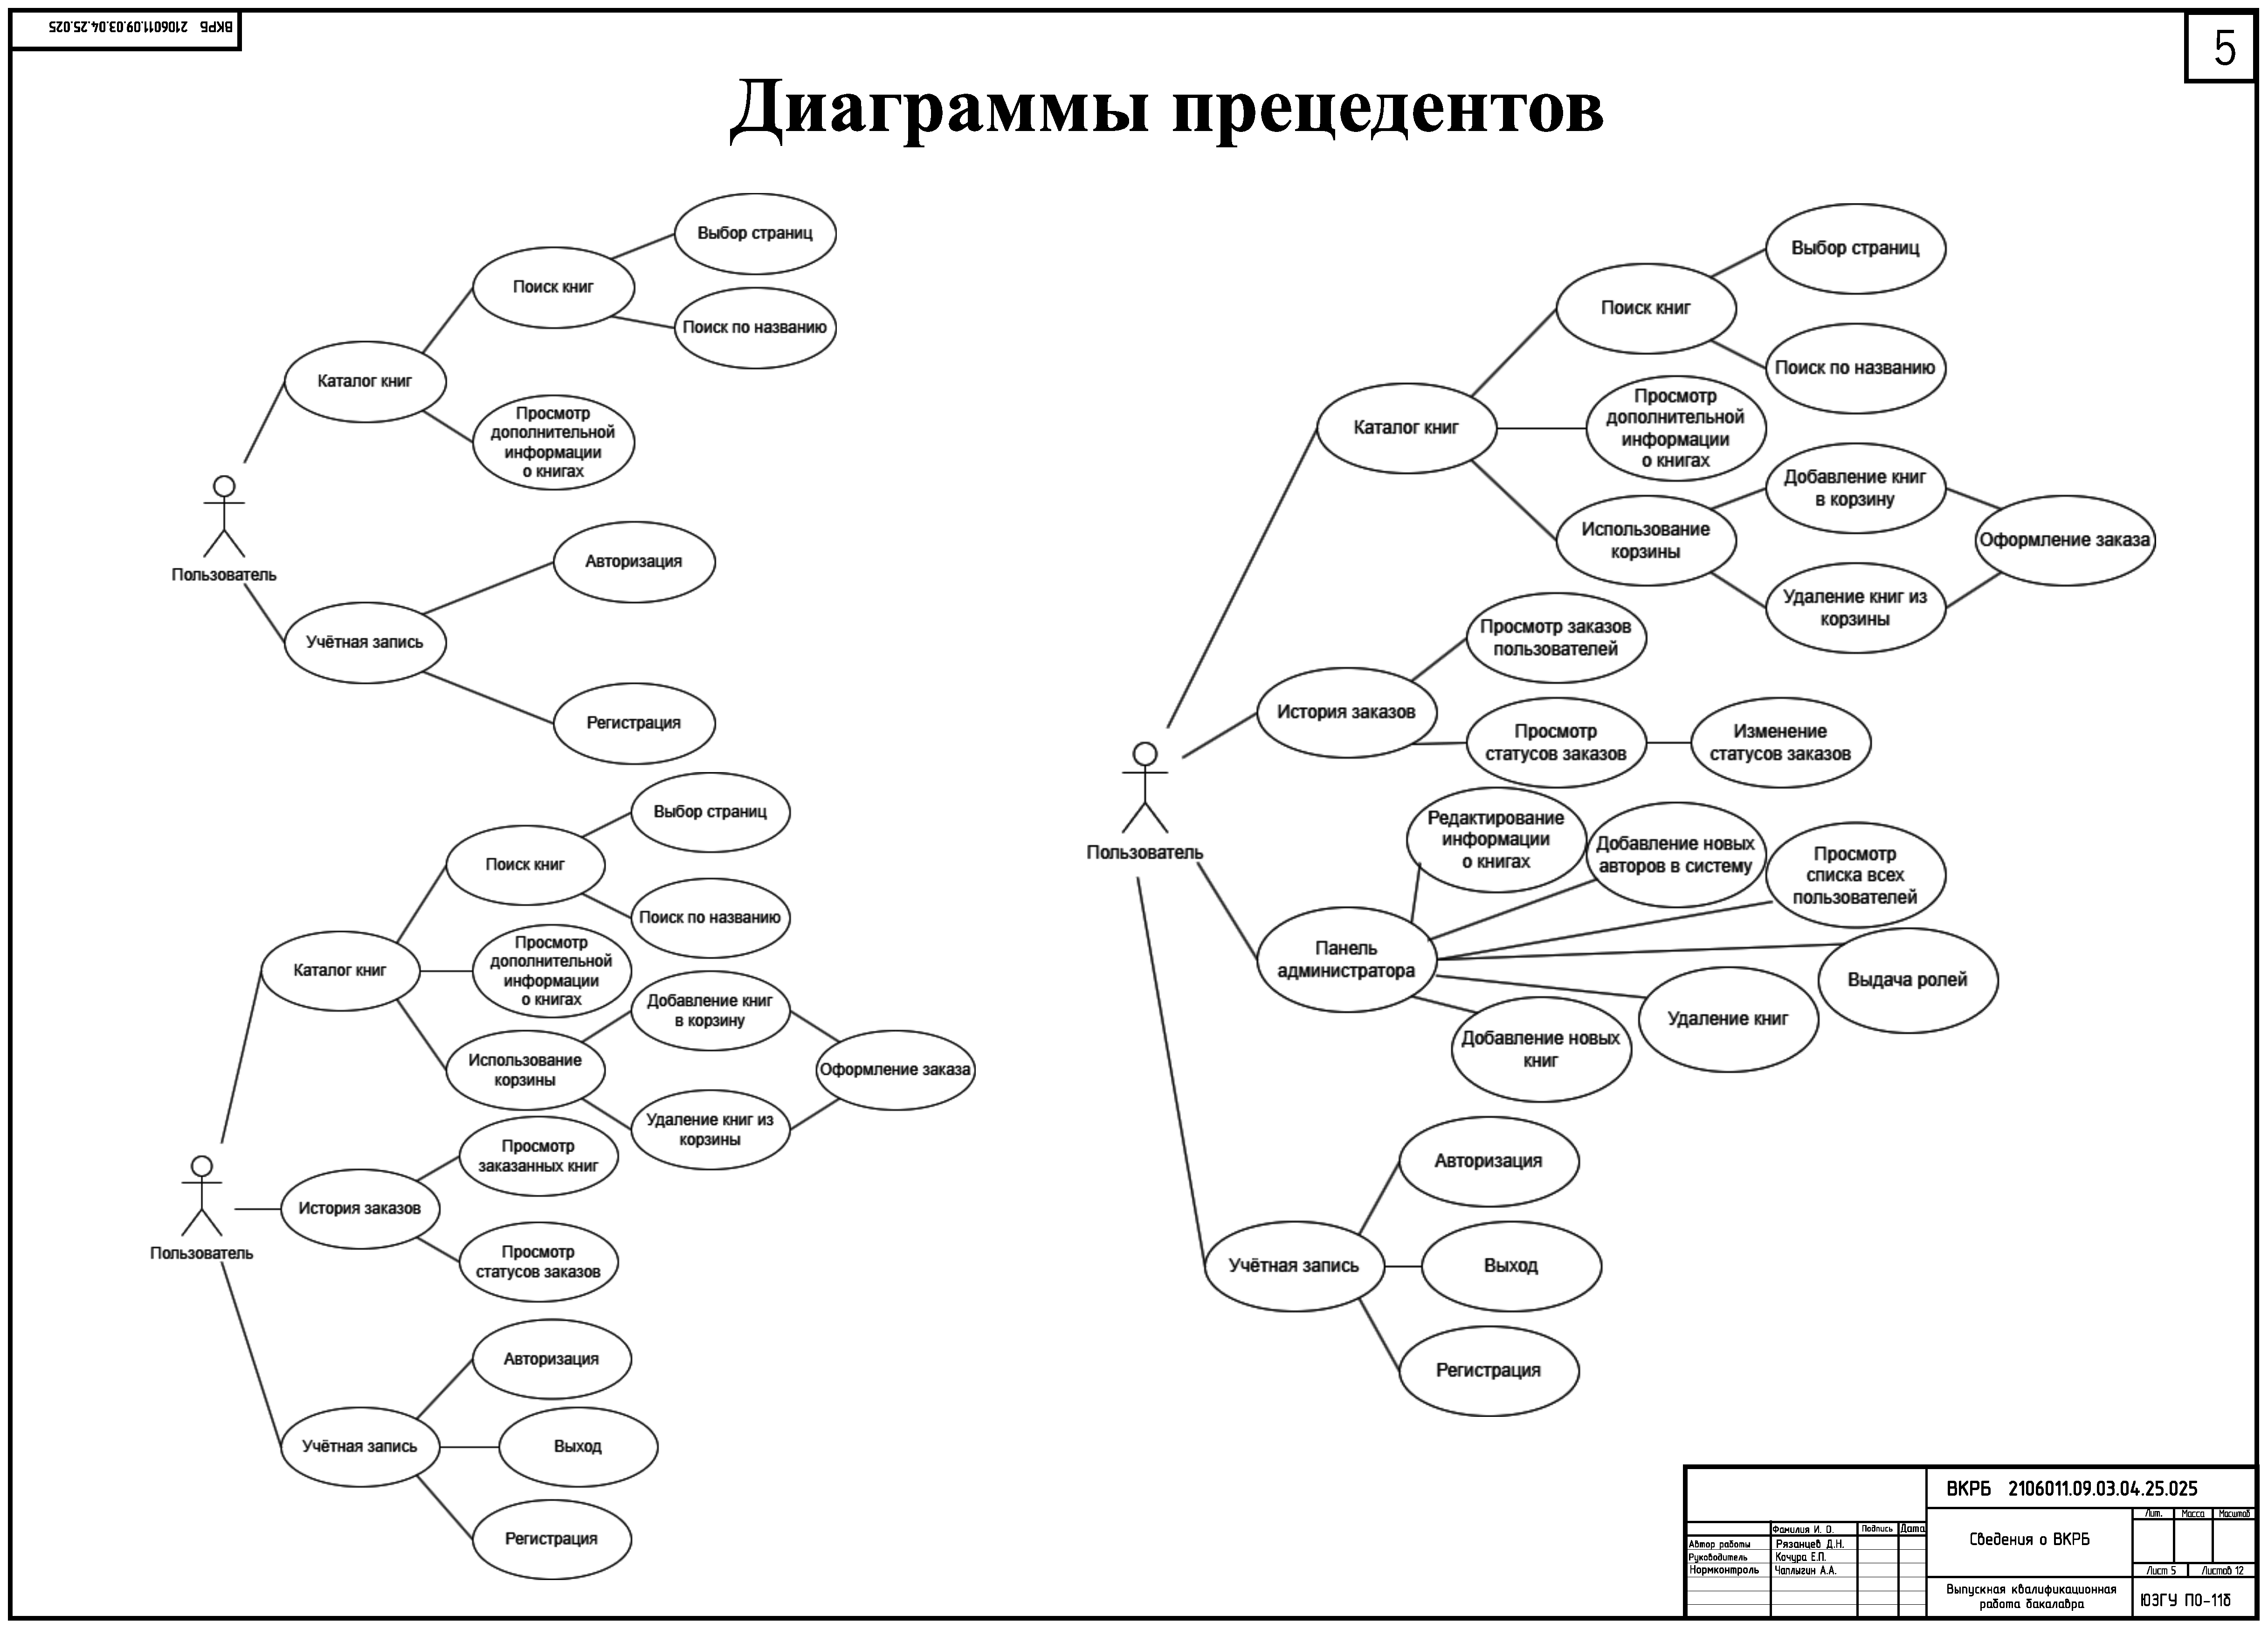
\includegraphics[width=0.82\linewidth]{5.eps}
	\заголовок{Диаграммы прецедентов}
	\label{pl5:image}      
\end{плакат}

\begin{плакат}
	
\includegraphics[width=0.82\linewidth]{6.eps}
	\заголовок{Архитектура интеллектуальной системы}
	\label{pl6:image}      
\end{плакат}

\begin{плакат}
	
\includegraphics[width=0.82\linewidth]{7.eps}
	\заголовок{Flask и REST API в системе}
	\label{pl7:image}      
\end{плакат}

\begin{плакат}
	
\includegraphics[width=0.82\linewidth]{8.eps}
	\заголовок{Интерфейс веб-приложения}
	\label{pl8:image}      
\end{плакат}

\begin{плакат}
	
\includegraphics[width=0.82\linewidth]{9.eps}
	\заголовок{Интерфейс веб-приложения}
	\label{pl9:image}      
\end{плакат}

\begin{плакат}
	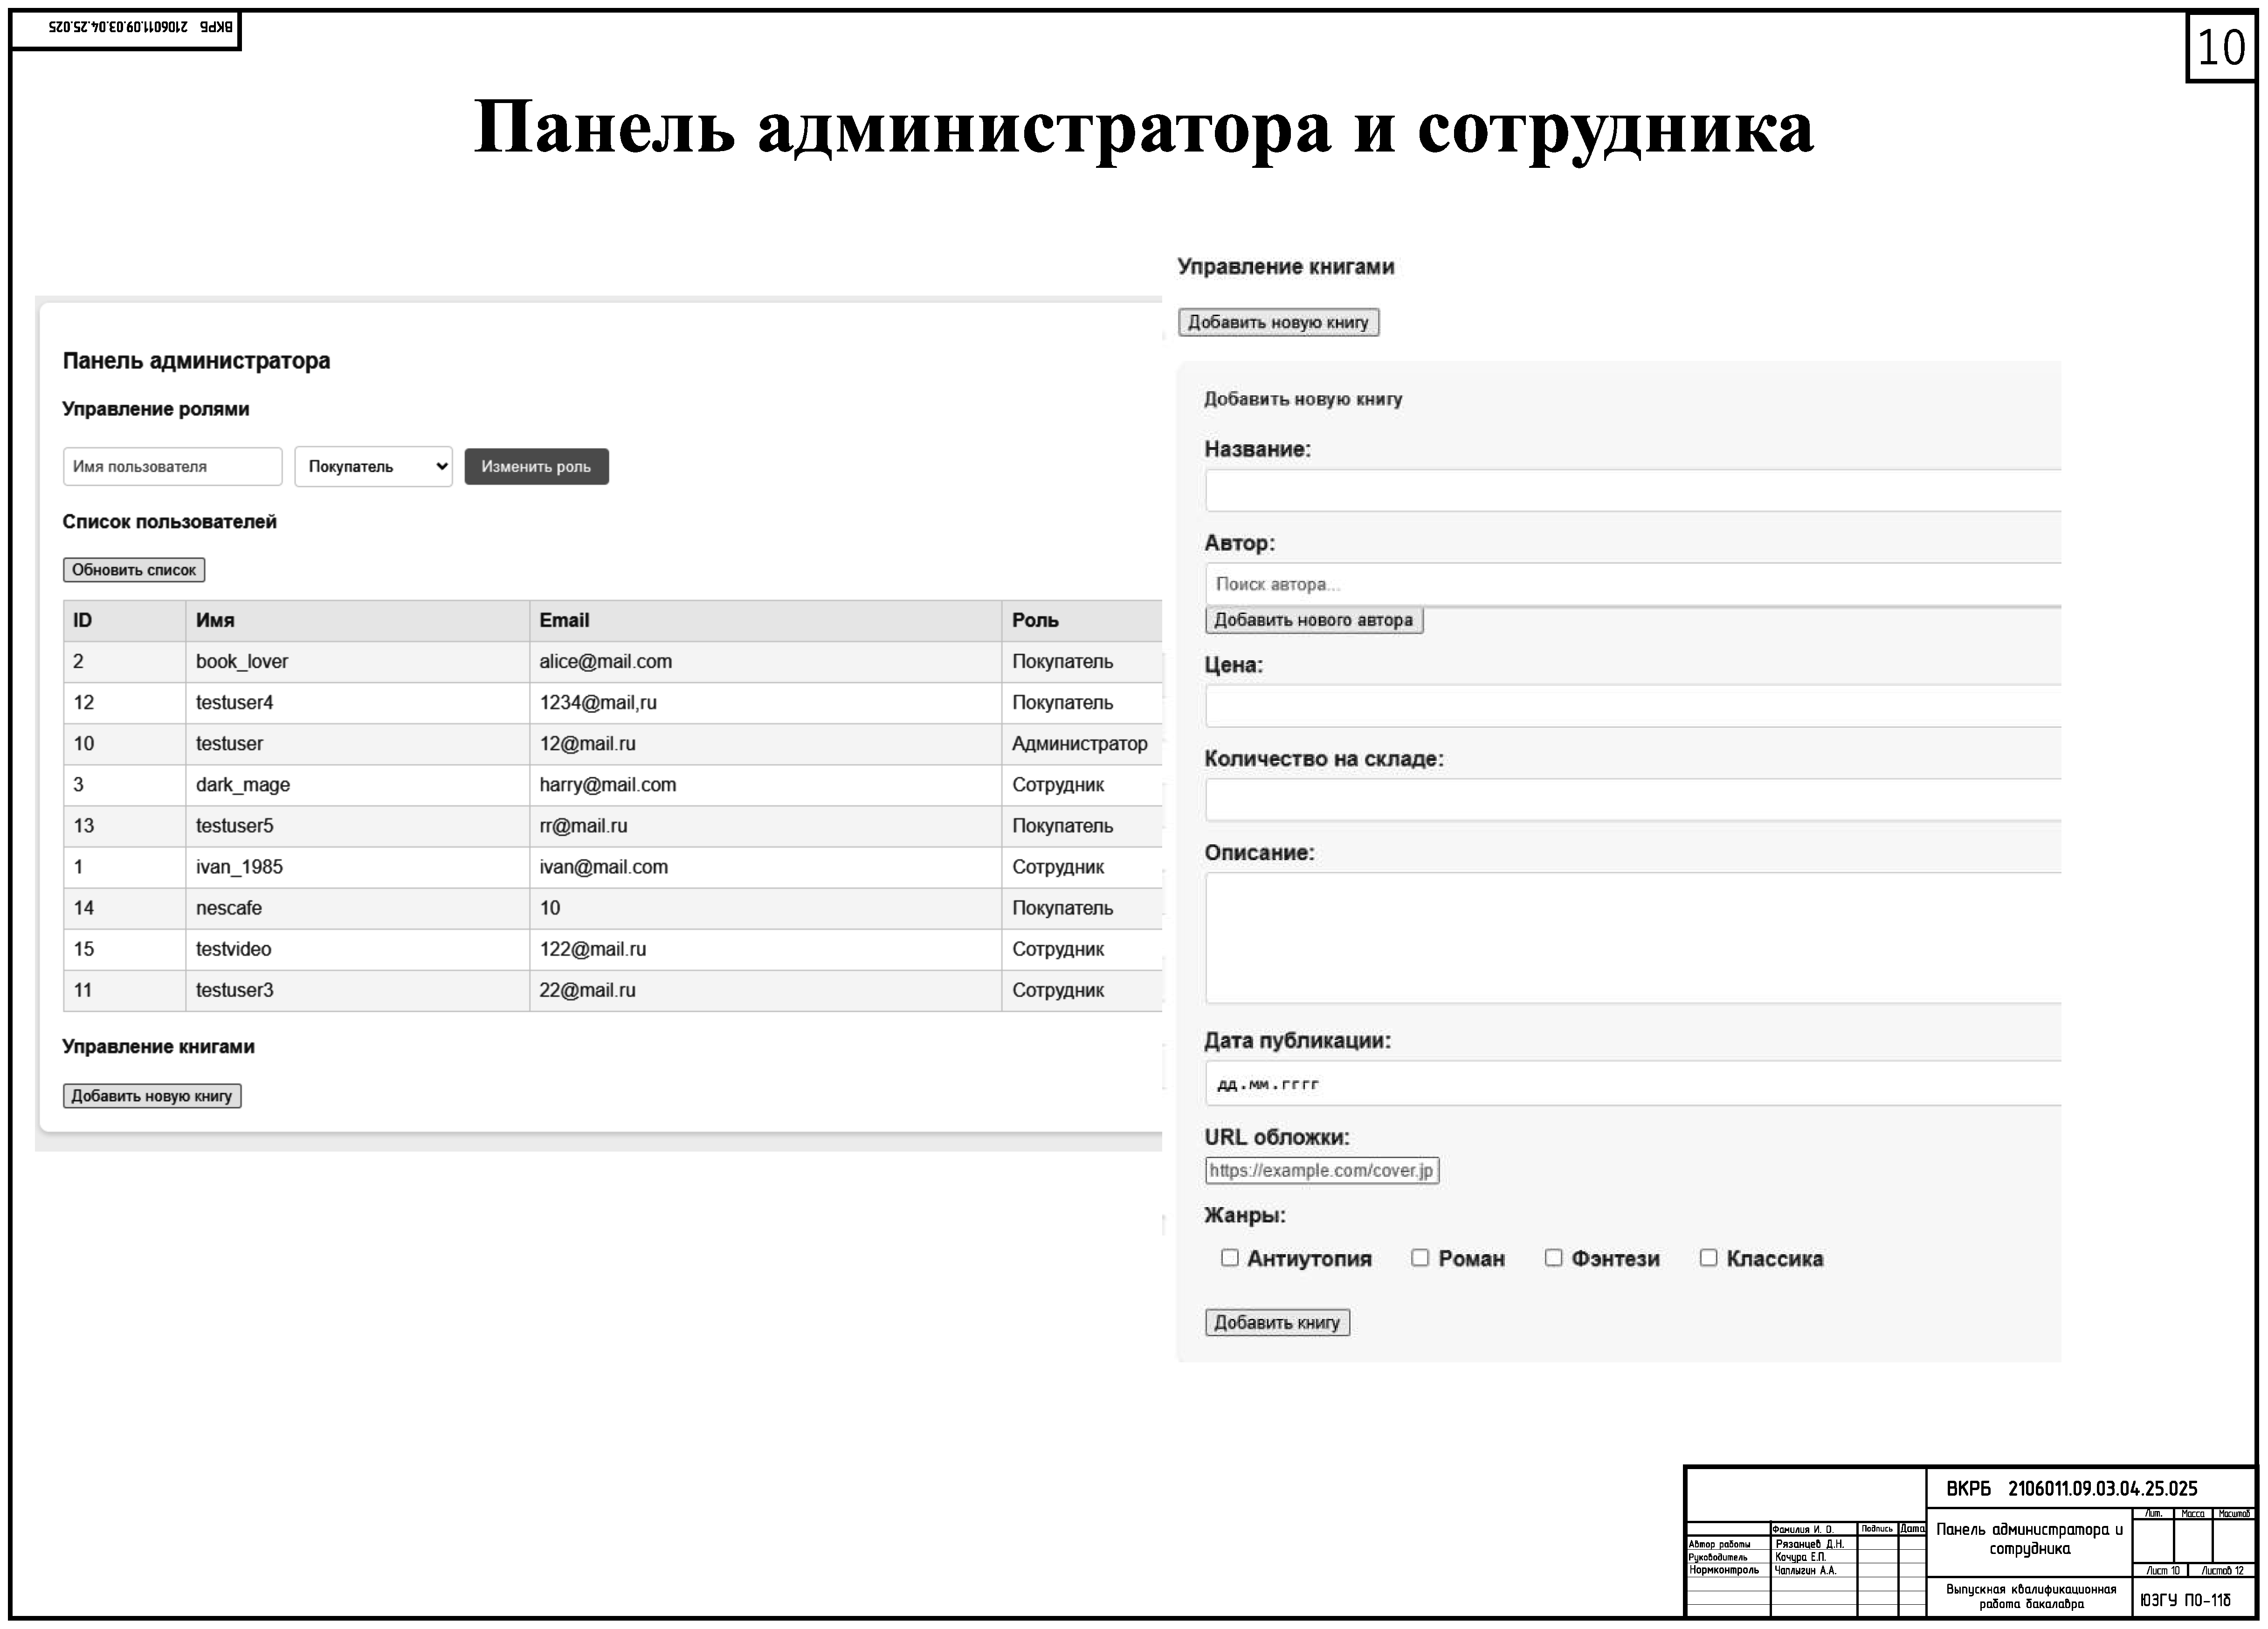
\includegraphics[width=0.82\linewidth]{10.eps}
	\заголовок{Панель администратора и сотрудника}
	\label{pl10:image}      
\end{плакат}

\begin{плакат}
	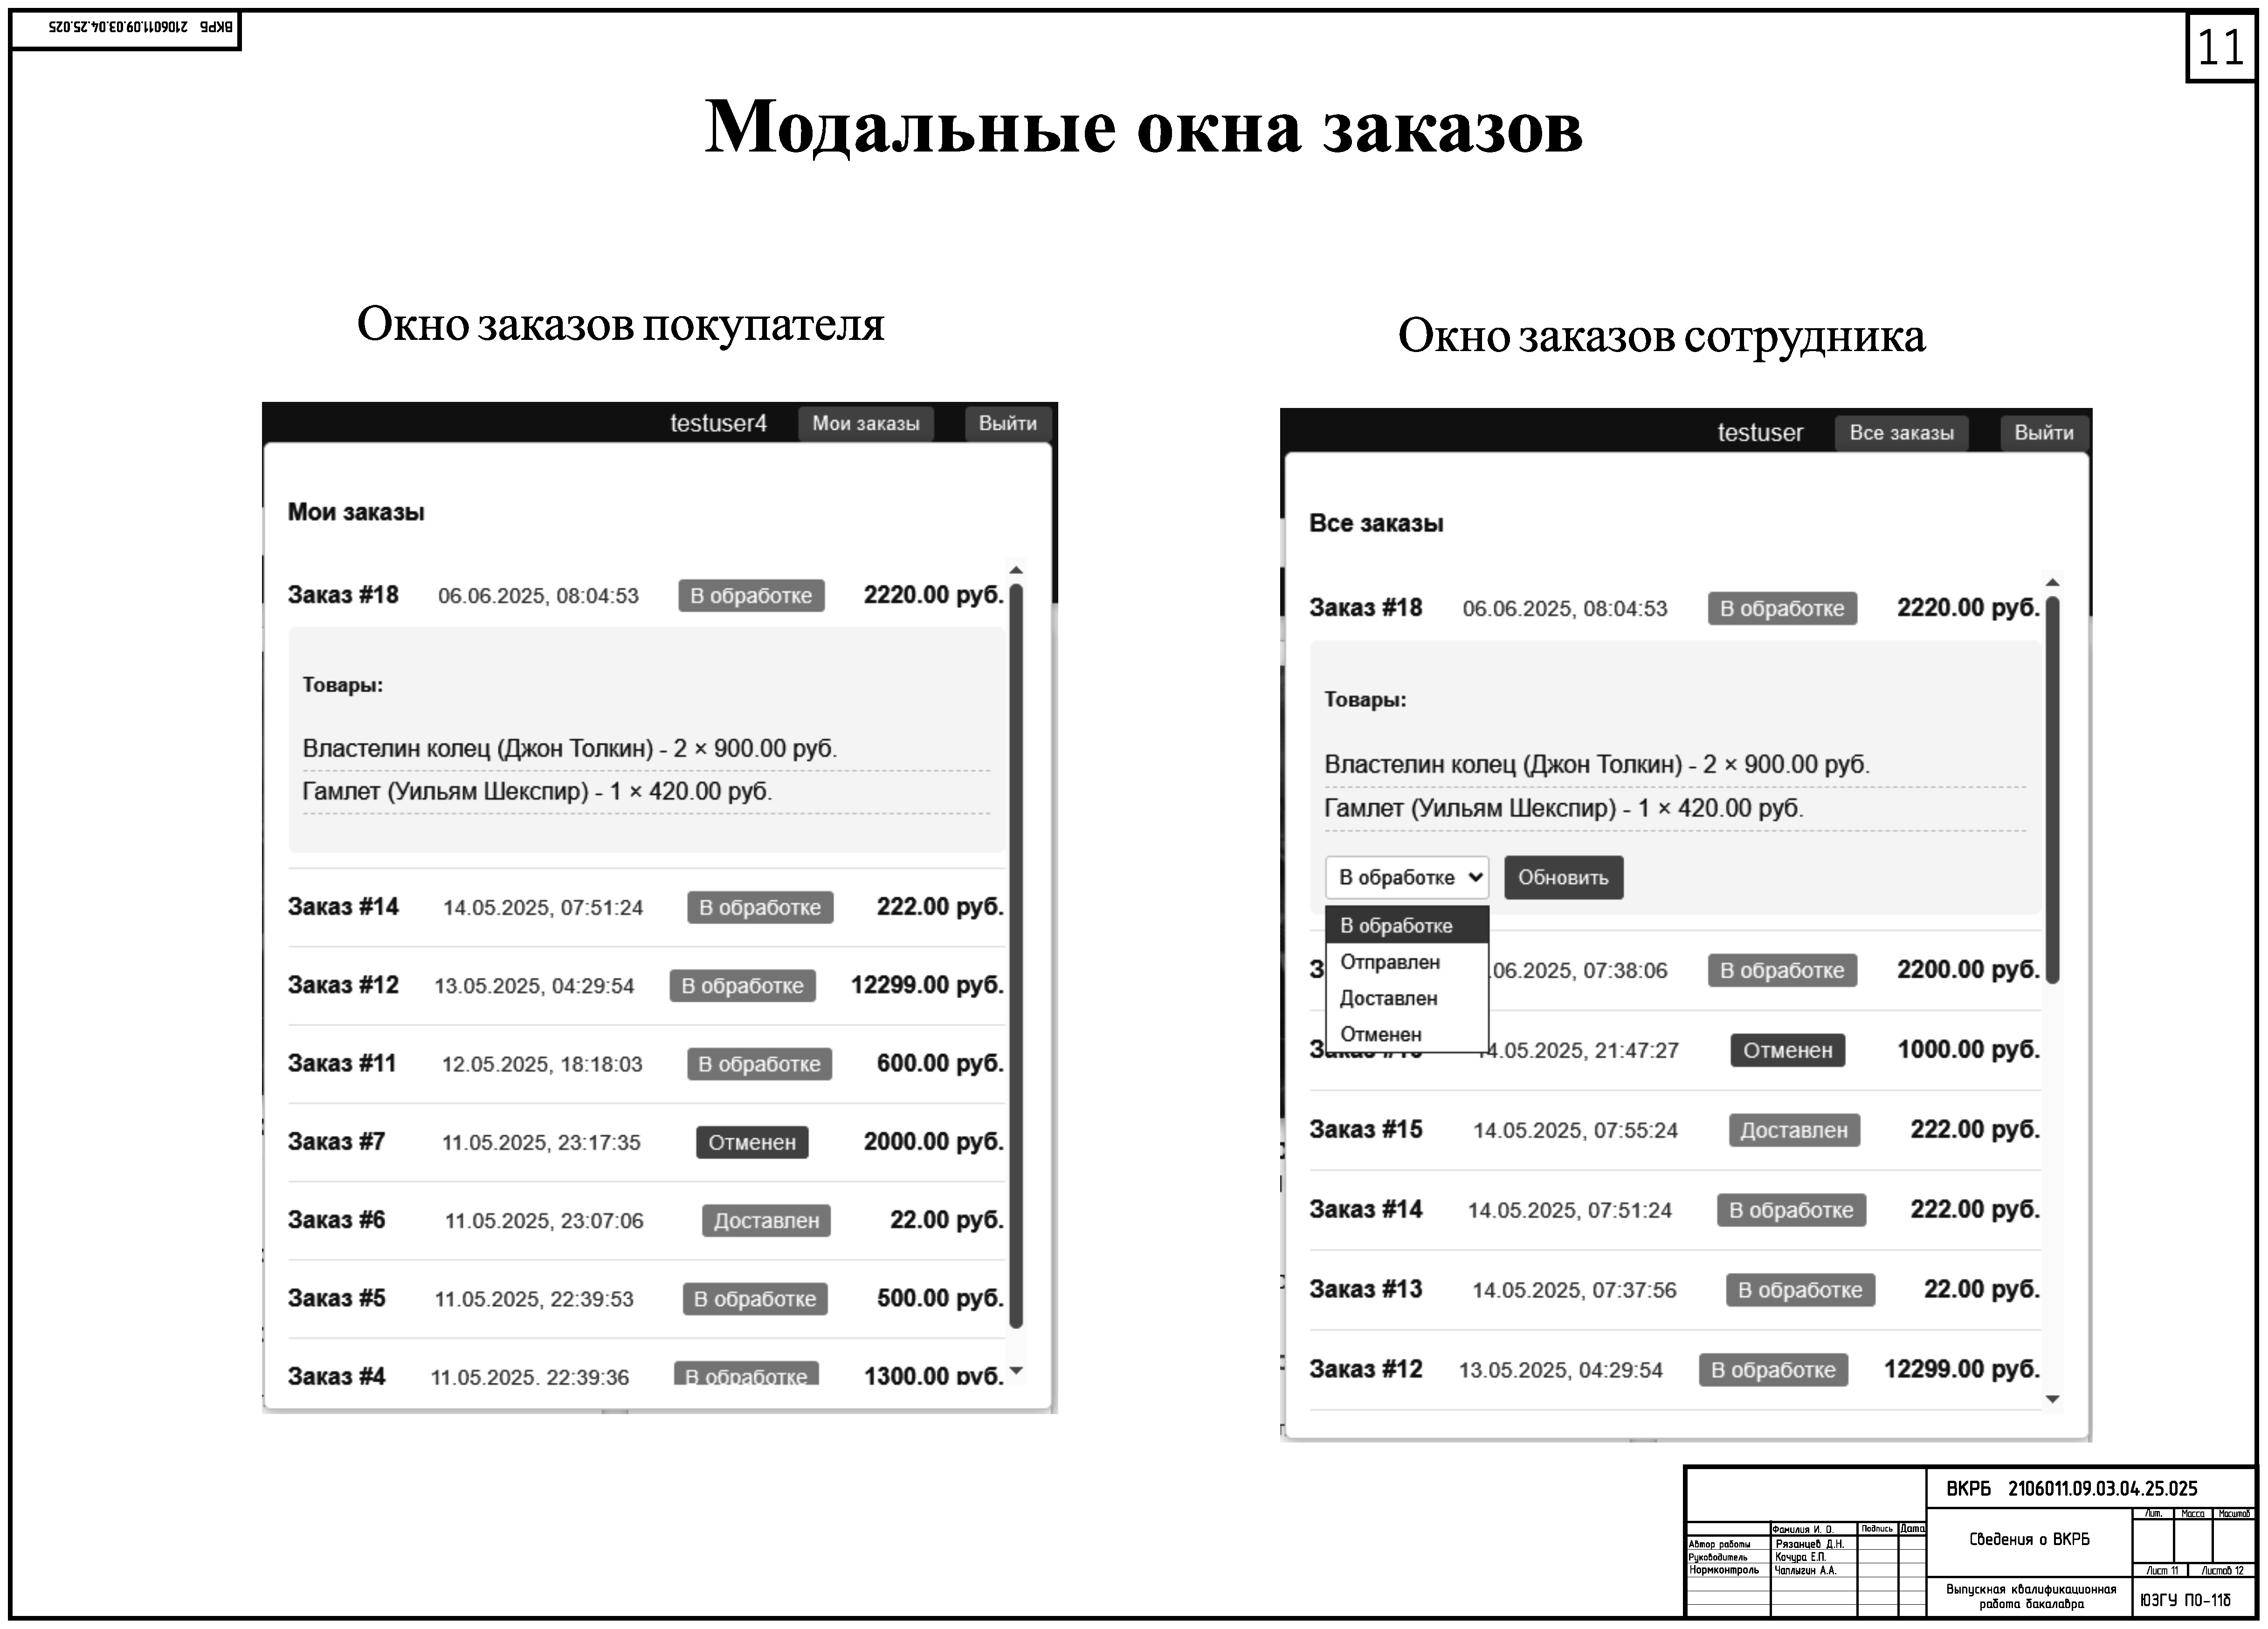
\includegraphics[width=0.82\linewidth]{11.eps}
	\заголовок{Модальные окна заказов}
	\label{pl11:image}      
\end{плакат}

\begin{плакат}
	
\includegraphics[width=0.82\linewidth]{12.eps}
	\заголовок{Заключение}
	\label{pl12:image}      
\end{плакат}












\end{landscape}}\fi
	\ifПрактика{}\else{\input{Код}}\fi
\end{document}
